
		\begin{figure}
			\centering
			\subfloat[SHREK]{
				\scalebox{.4}{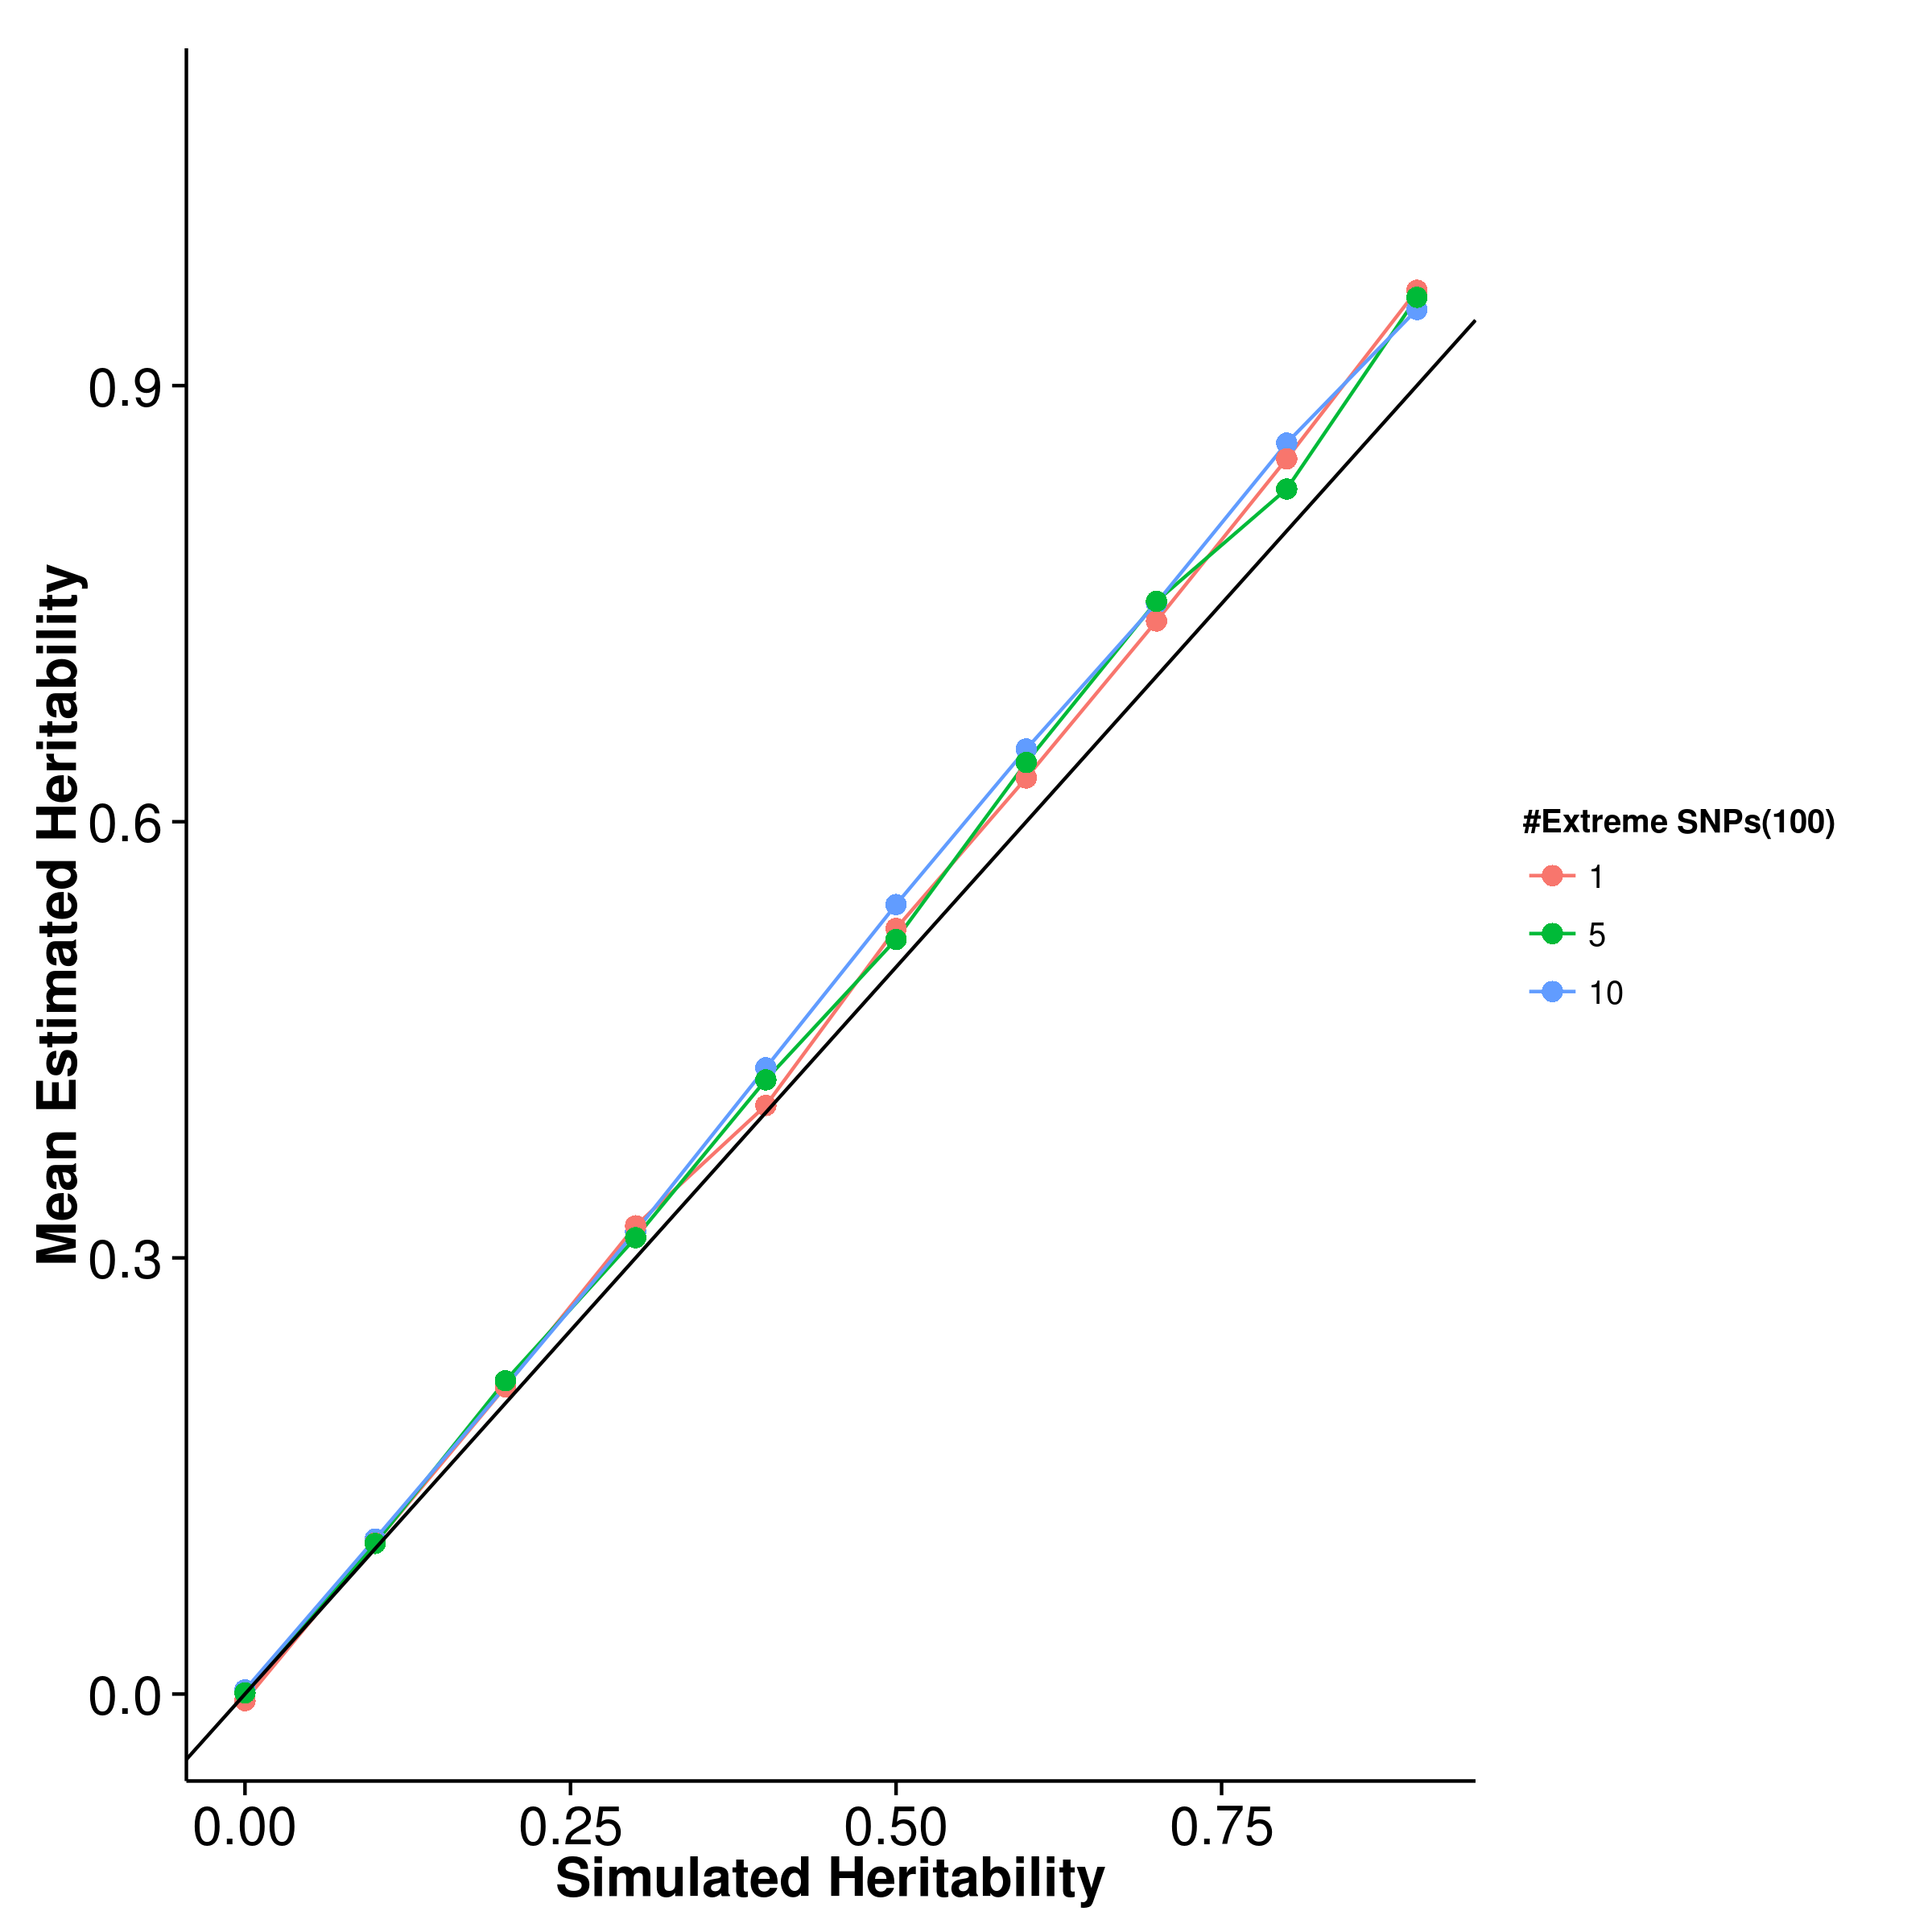
\includegraphics{figure/he_summary/extreme_100c/shrek_QtE_Rand_mean.png}}
				\label{fig:shrekQtEx100cMean}
			}
			\subfloat[GCTA]{
				\scalebox{.4}{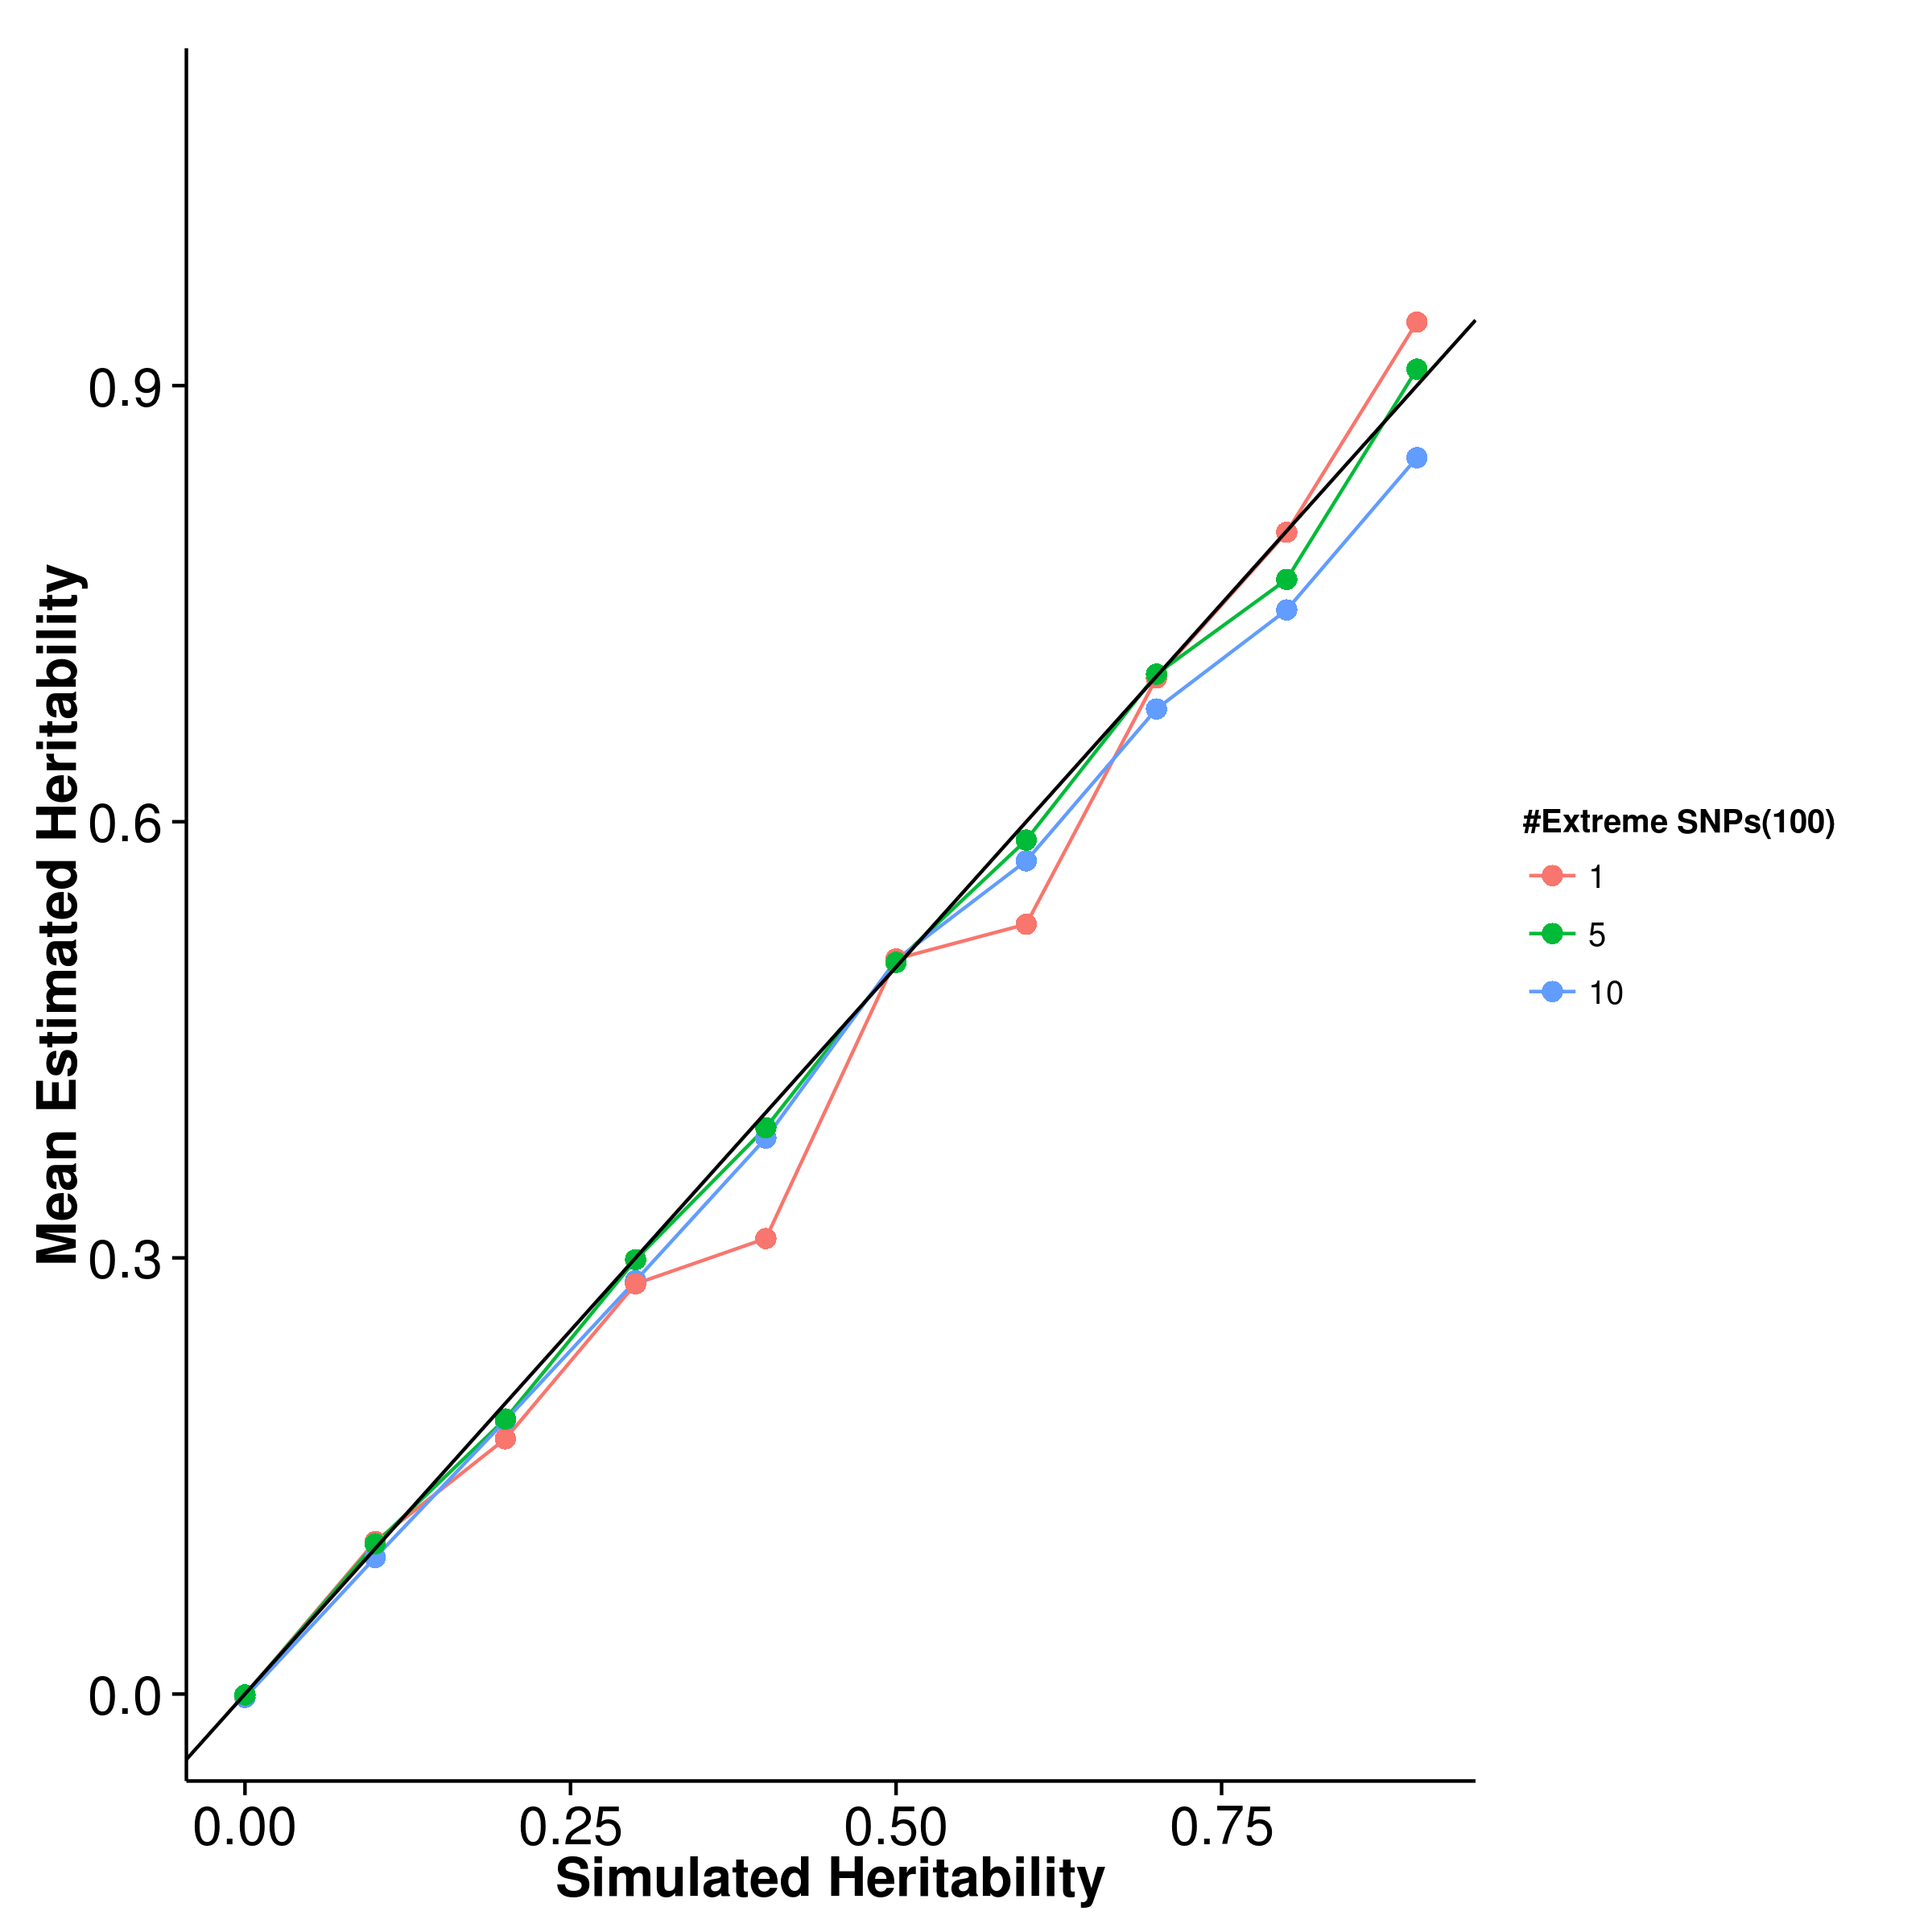
\includegraphics{figure/he_summary/extreme_100c/gcta_QtE_Rand_mean.png}}
				\label{fig:gctaQtEx100cMean}
			}\\
			\subfloat[LDSC with fix intercept]{
				\scalebox{.4}{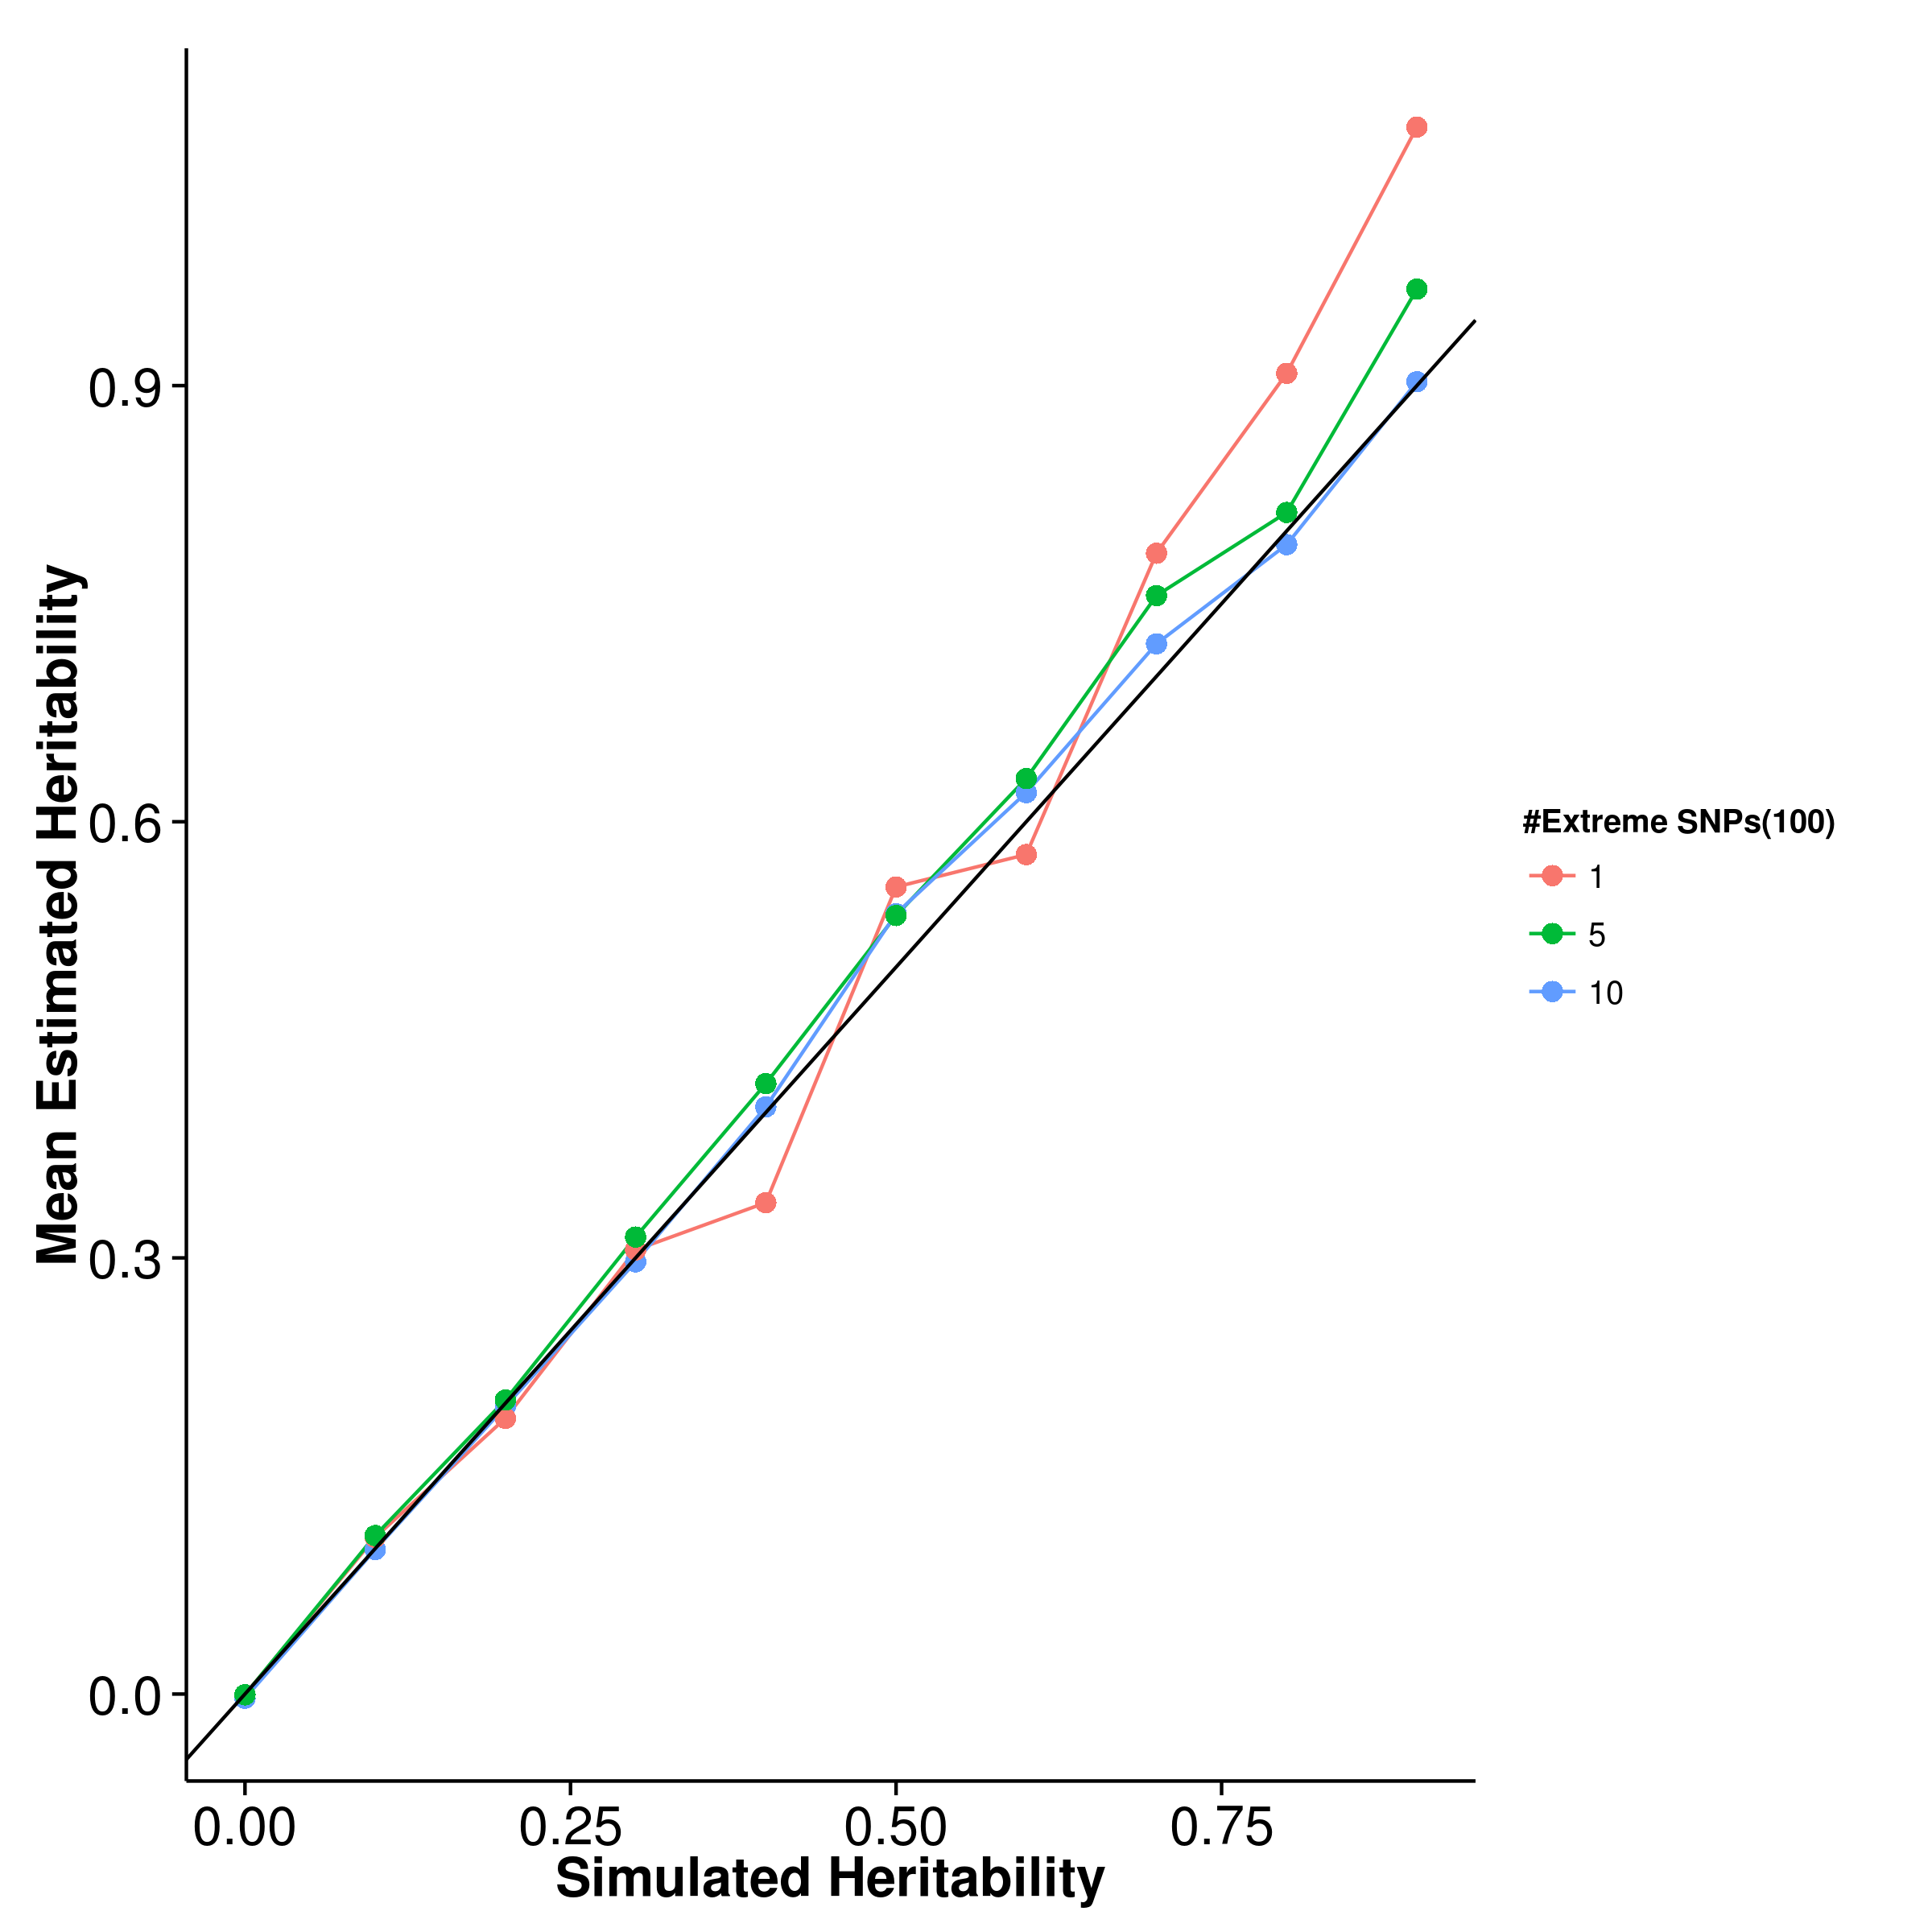
\includegraphics{figure/he_summary/extreme_100c/ldsc_QtE_Rand_mean.png}}
				\label{fig:ldscQtEx100cMean}
			}
			\subfloat[LDSC with intercept estimation]{
				
				\scalebox{.4}{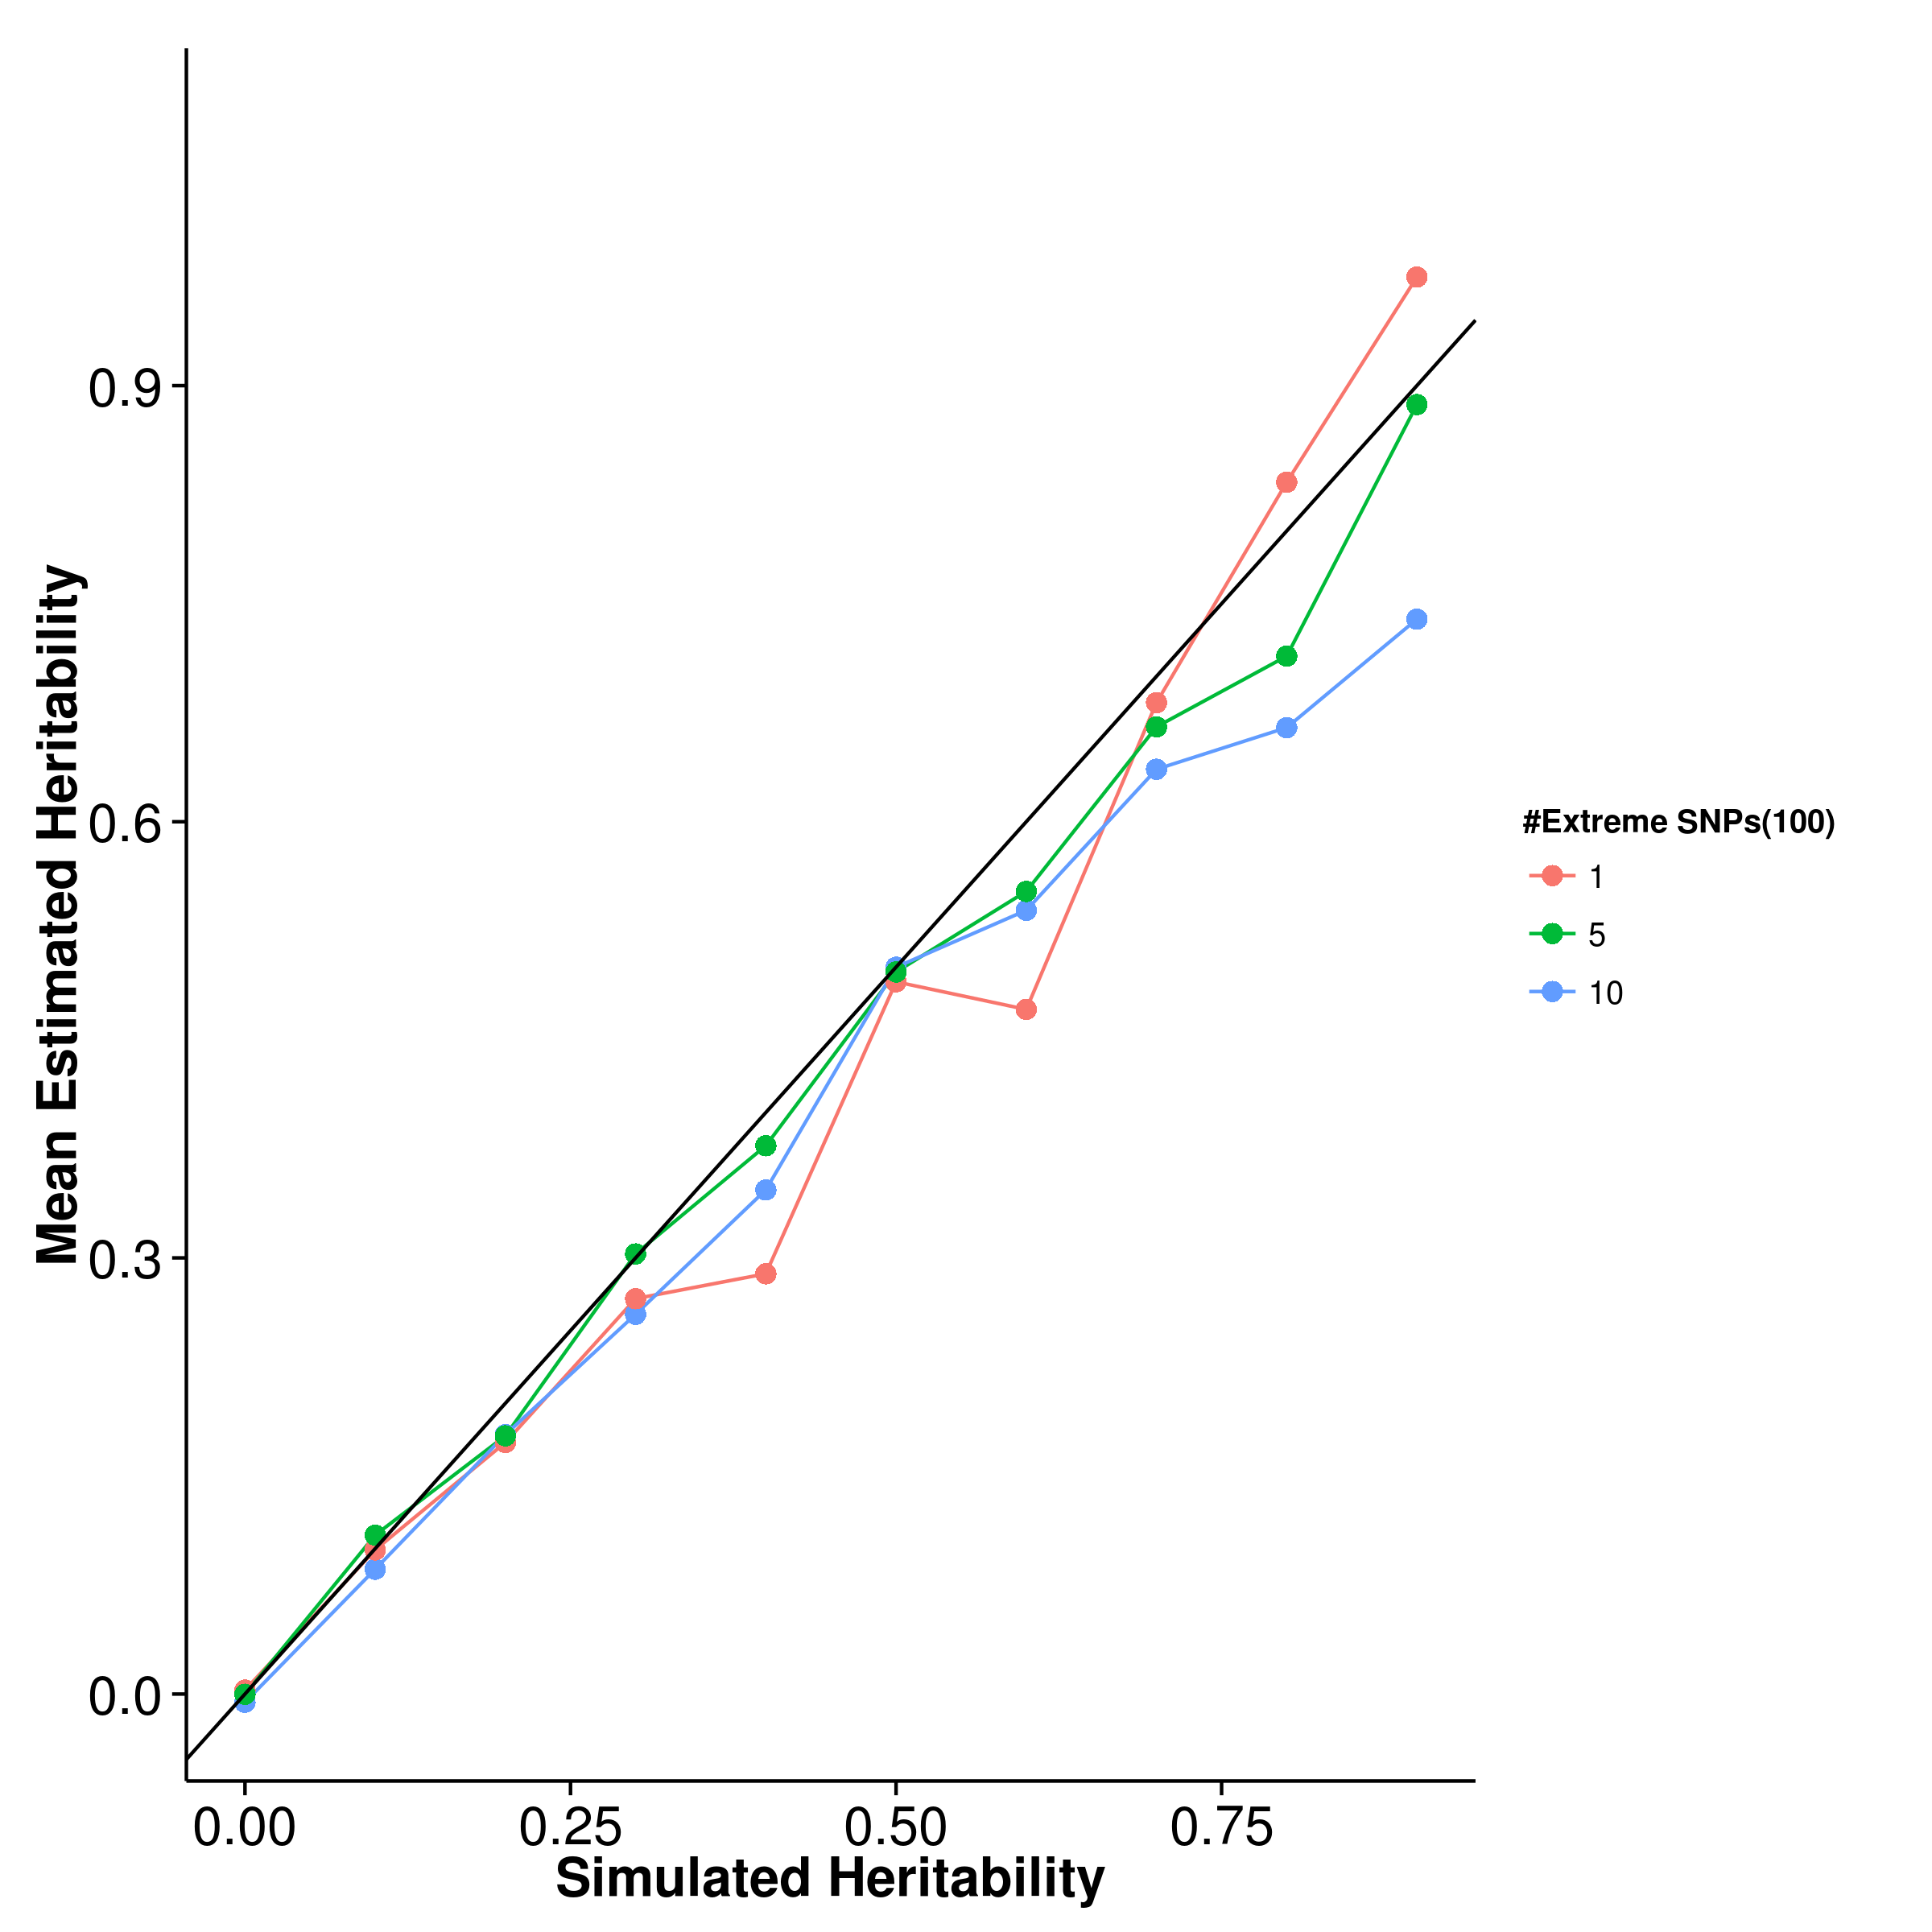
\includegraphics{figure/he_summary/extreme_100c/ldscIn_QtE_Rand_mean.png}}
				\label{fig:ldscInQtEx100cMean}
			}
			\caption[Mean of Extreme Effect Size Simulation Result]
			{Mean of results from quantitative trait simulation with extreme effect size simulation.
				It was observed that the mean estimation of heritability of \gls{shrek} is not affected by the number of \gls{SNP}(s) with large effect but with slight upward bias.
				On the other hand, the mean estimation of \gls{ldsc} and \gls{gcta} seems to fluctuate with respect to the simulated heritability.
				} 
			\label{fig:QtEx100cMean}
		\end{figure}
		
		\begin{figure}
			\centering
			\subfloat[SHREK]{
				\scalebox{.4}{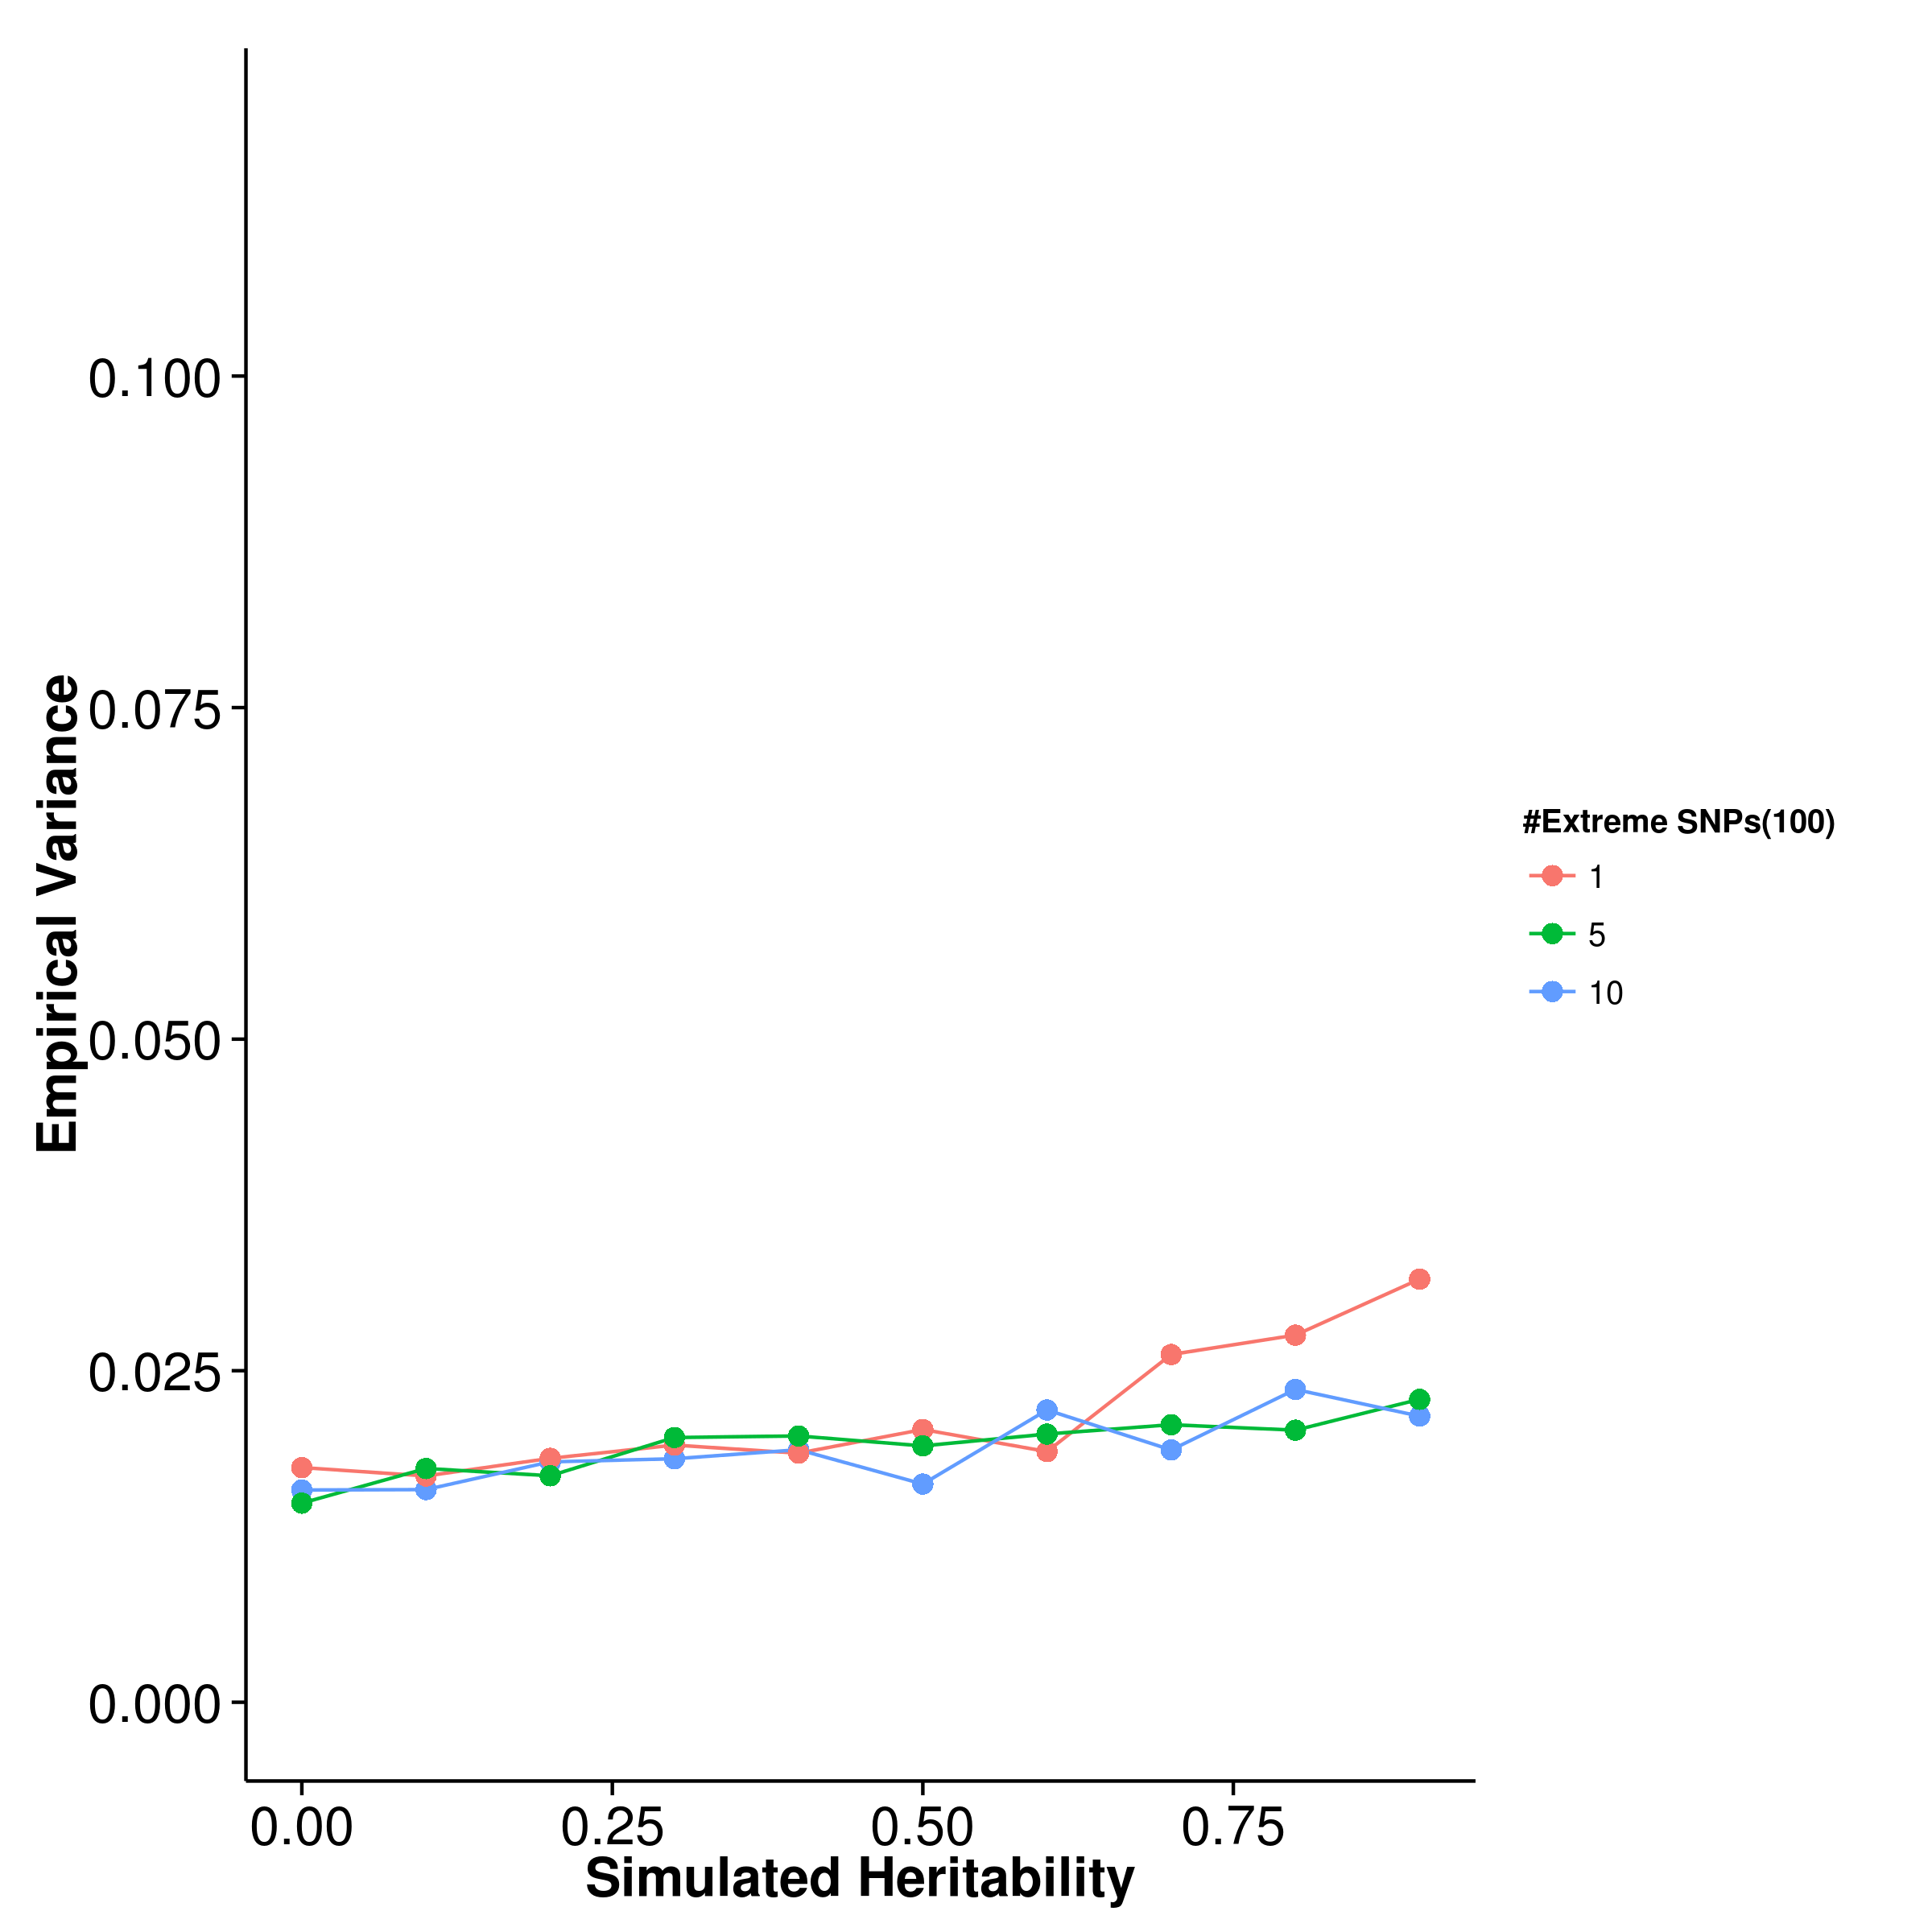
\includegraphics{figure/he_summary/extreme_100c/shrek_QtE_Rand_sd.png}}
				\label{fig:shrekQtEx100cVar}
			}
			\subfloat[GCTA]{
				\scalebox{.4}{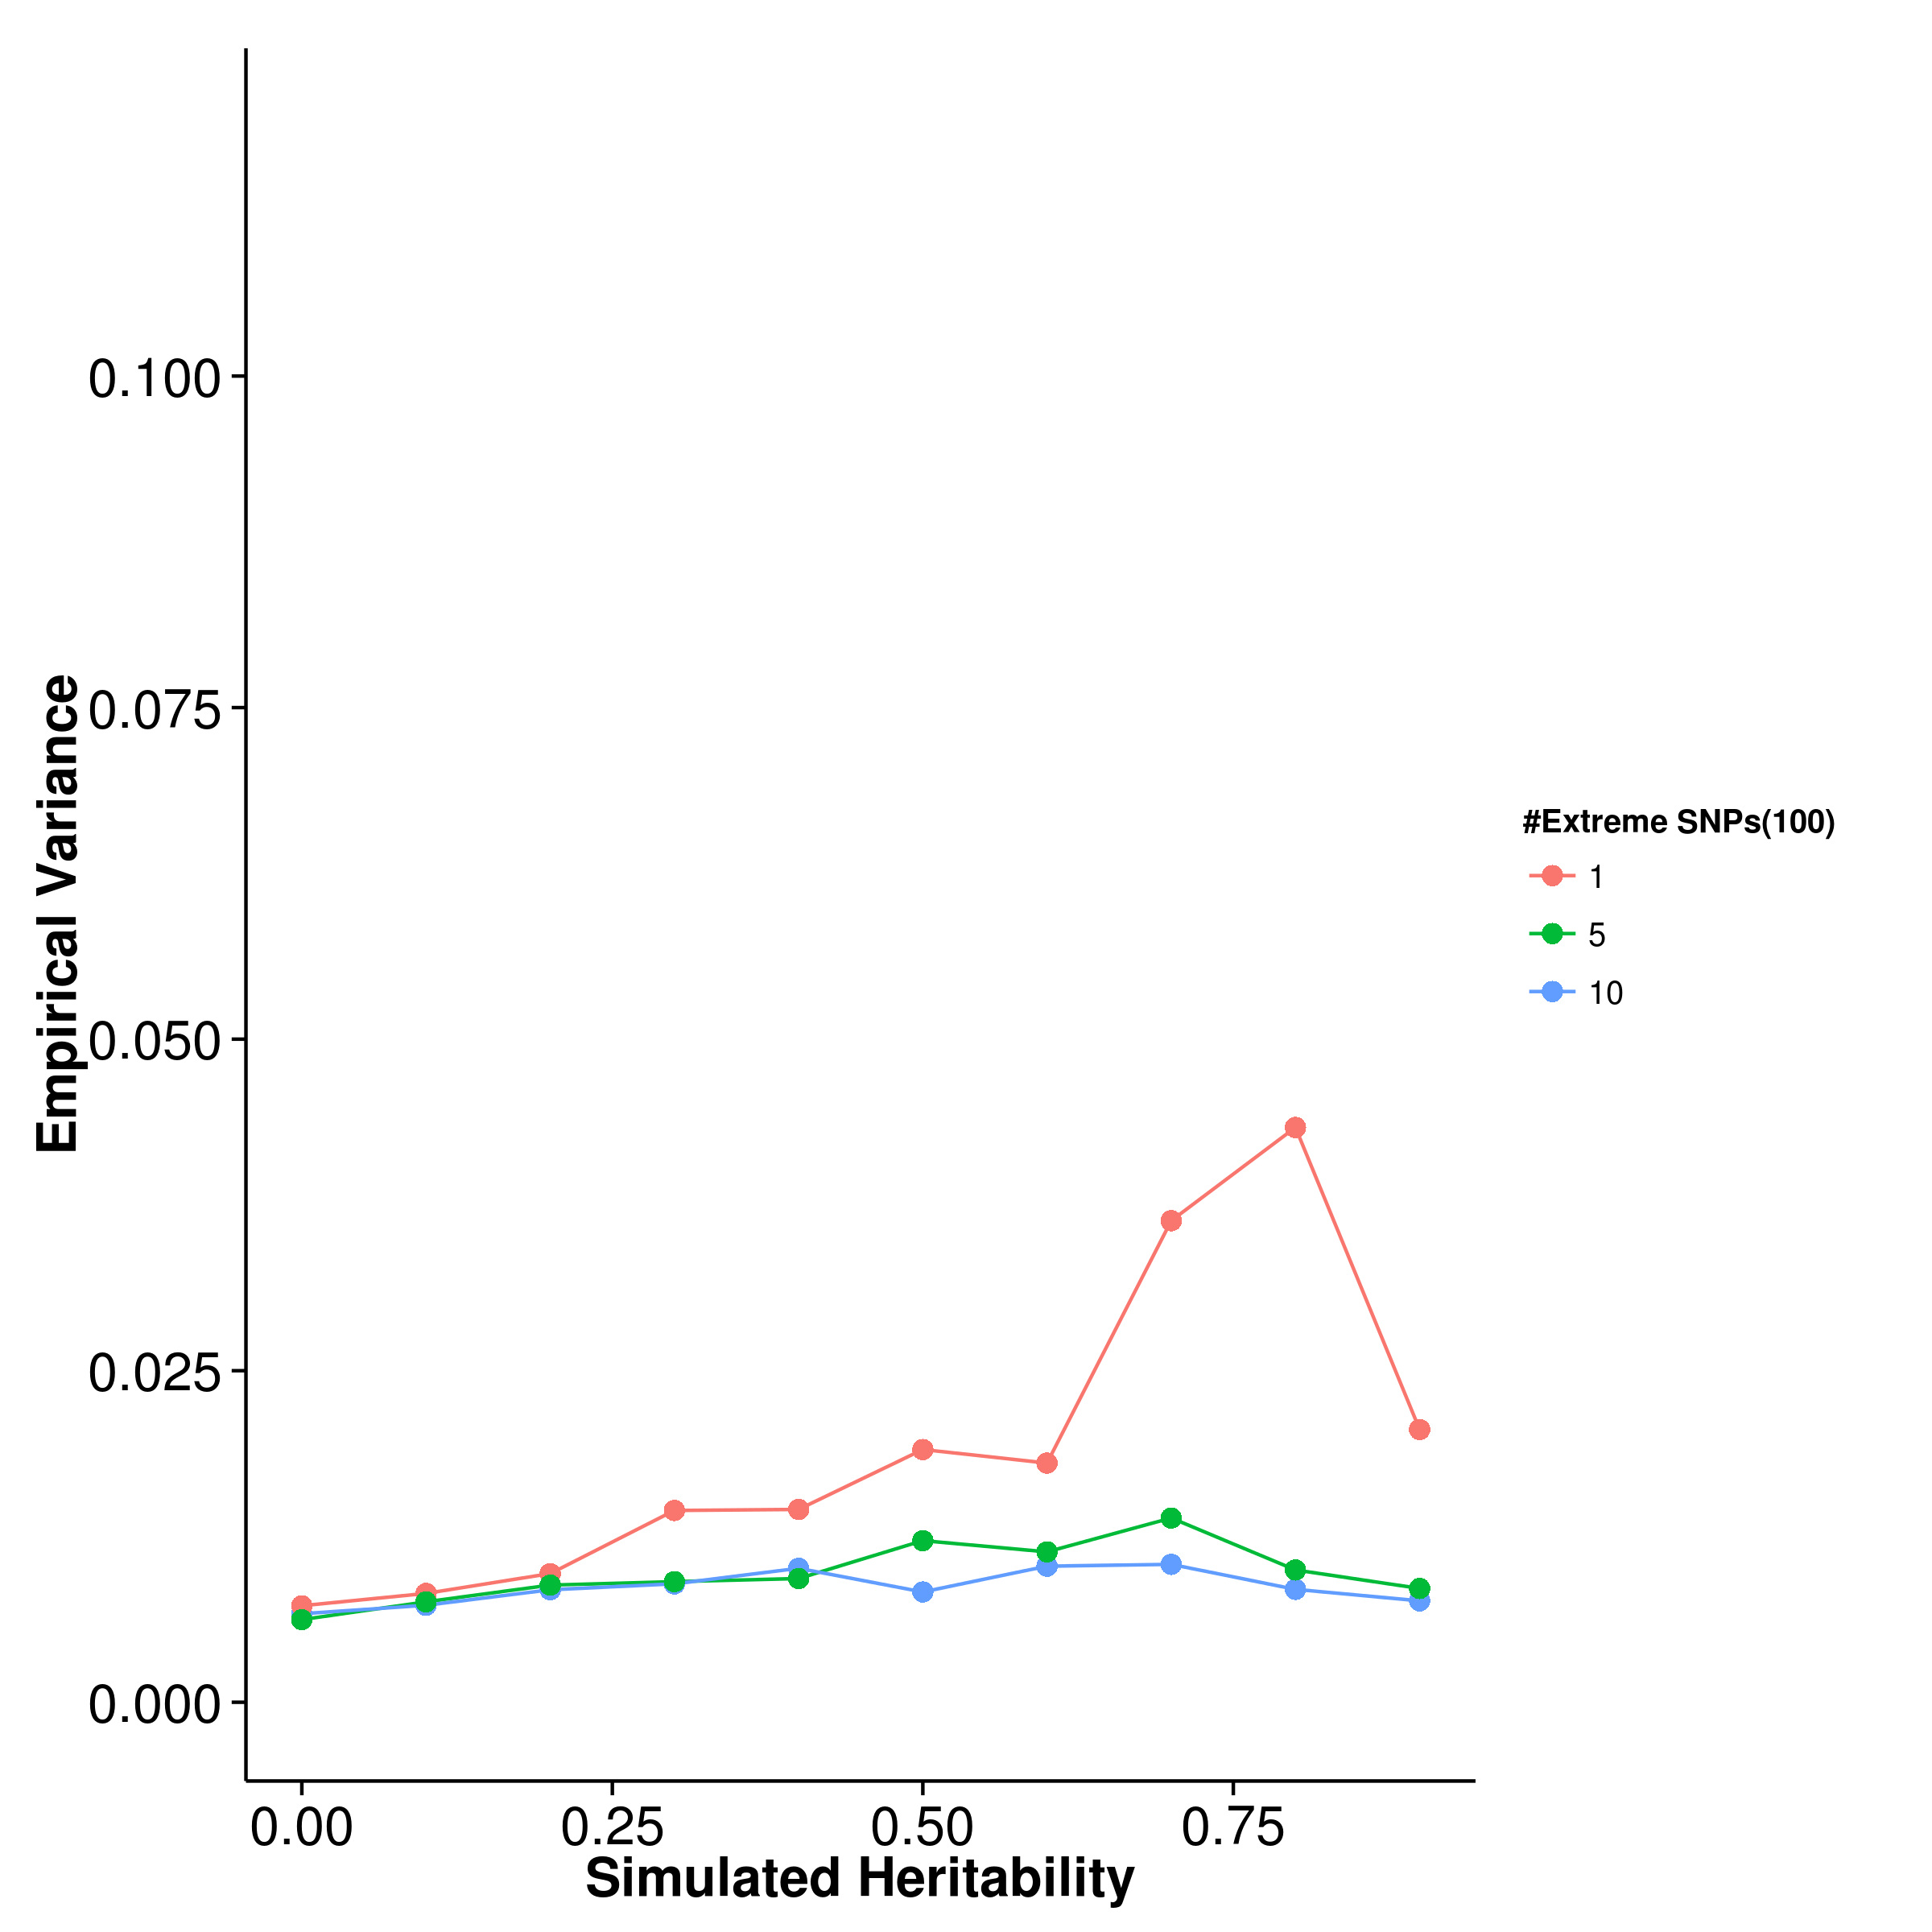
\includegraphics{figure/he_summary/extreme_100c/gcta_QtE_Rand_sd.png}}
				\label{fig:gctaQtEx100cVar}
			}\\
			\subfloat[LDSC with fix intercept]{
				\scalebox{.4}{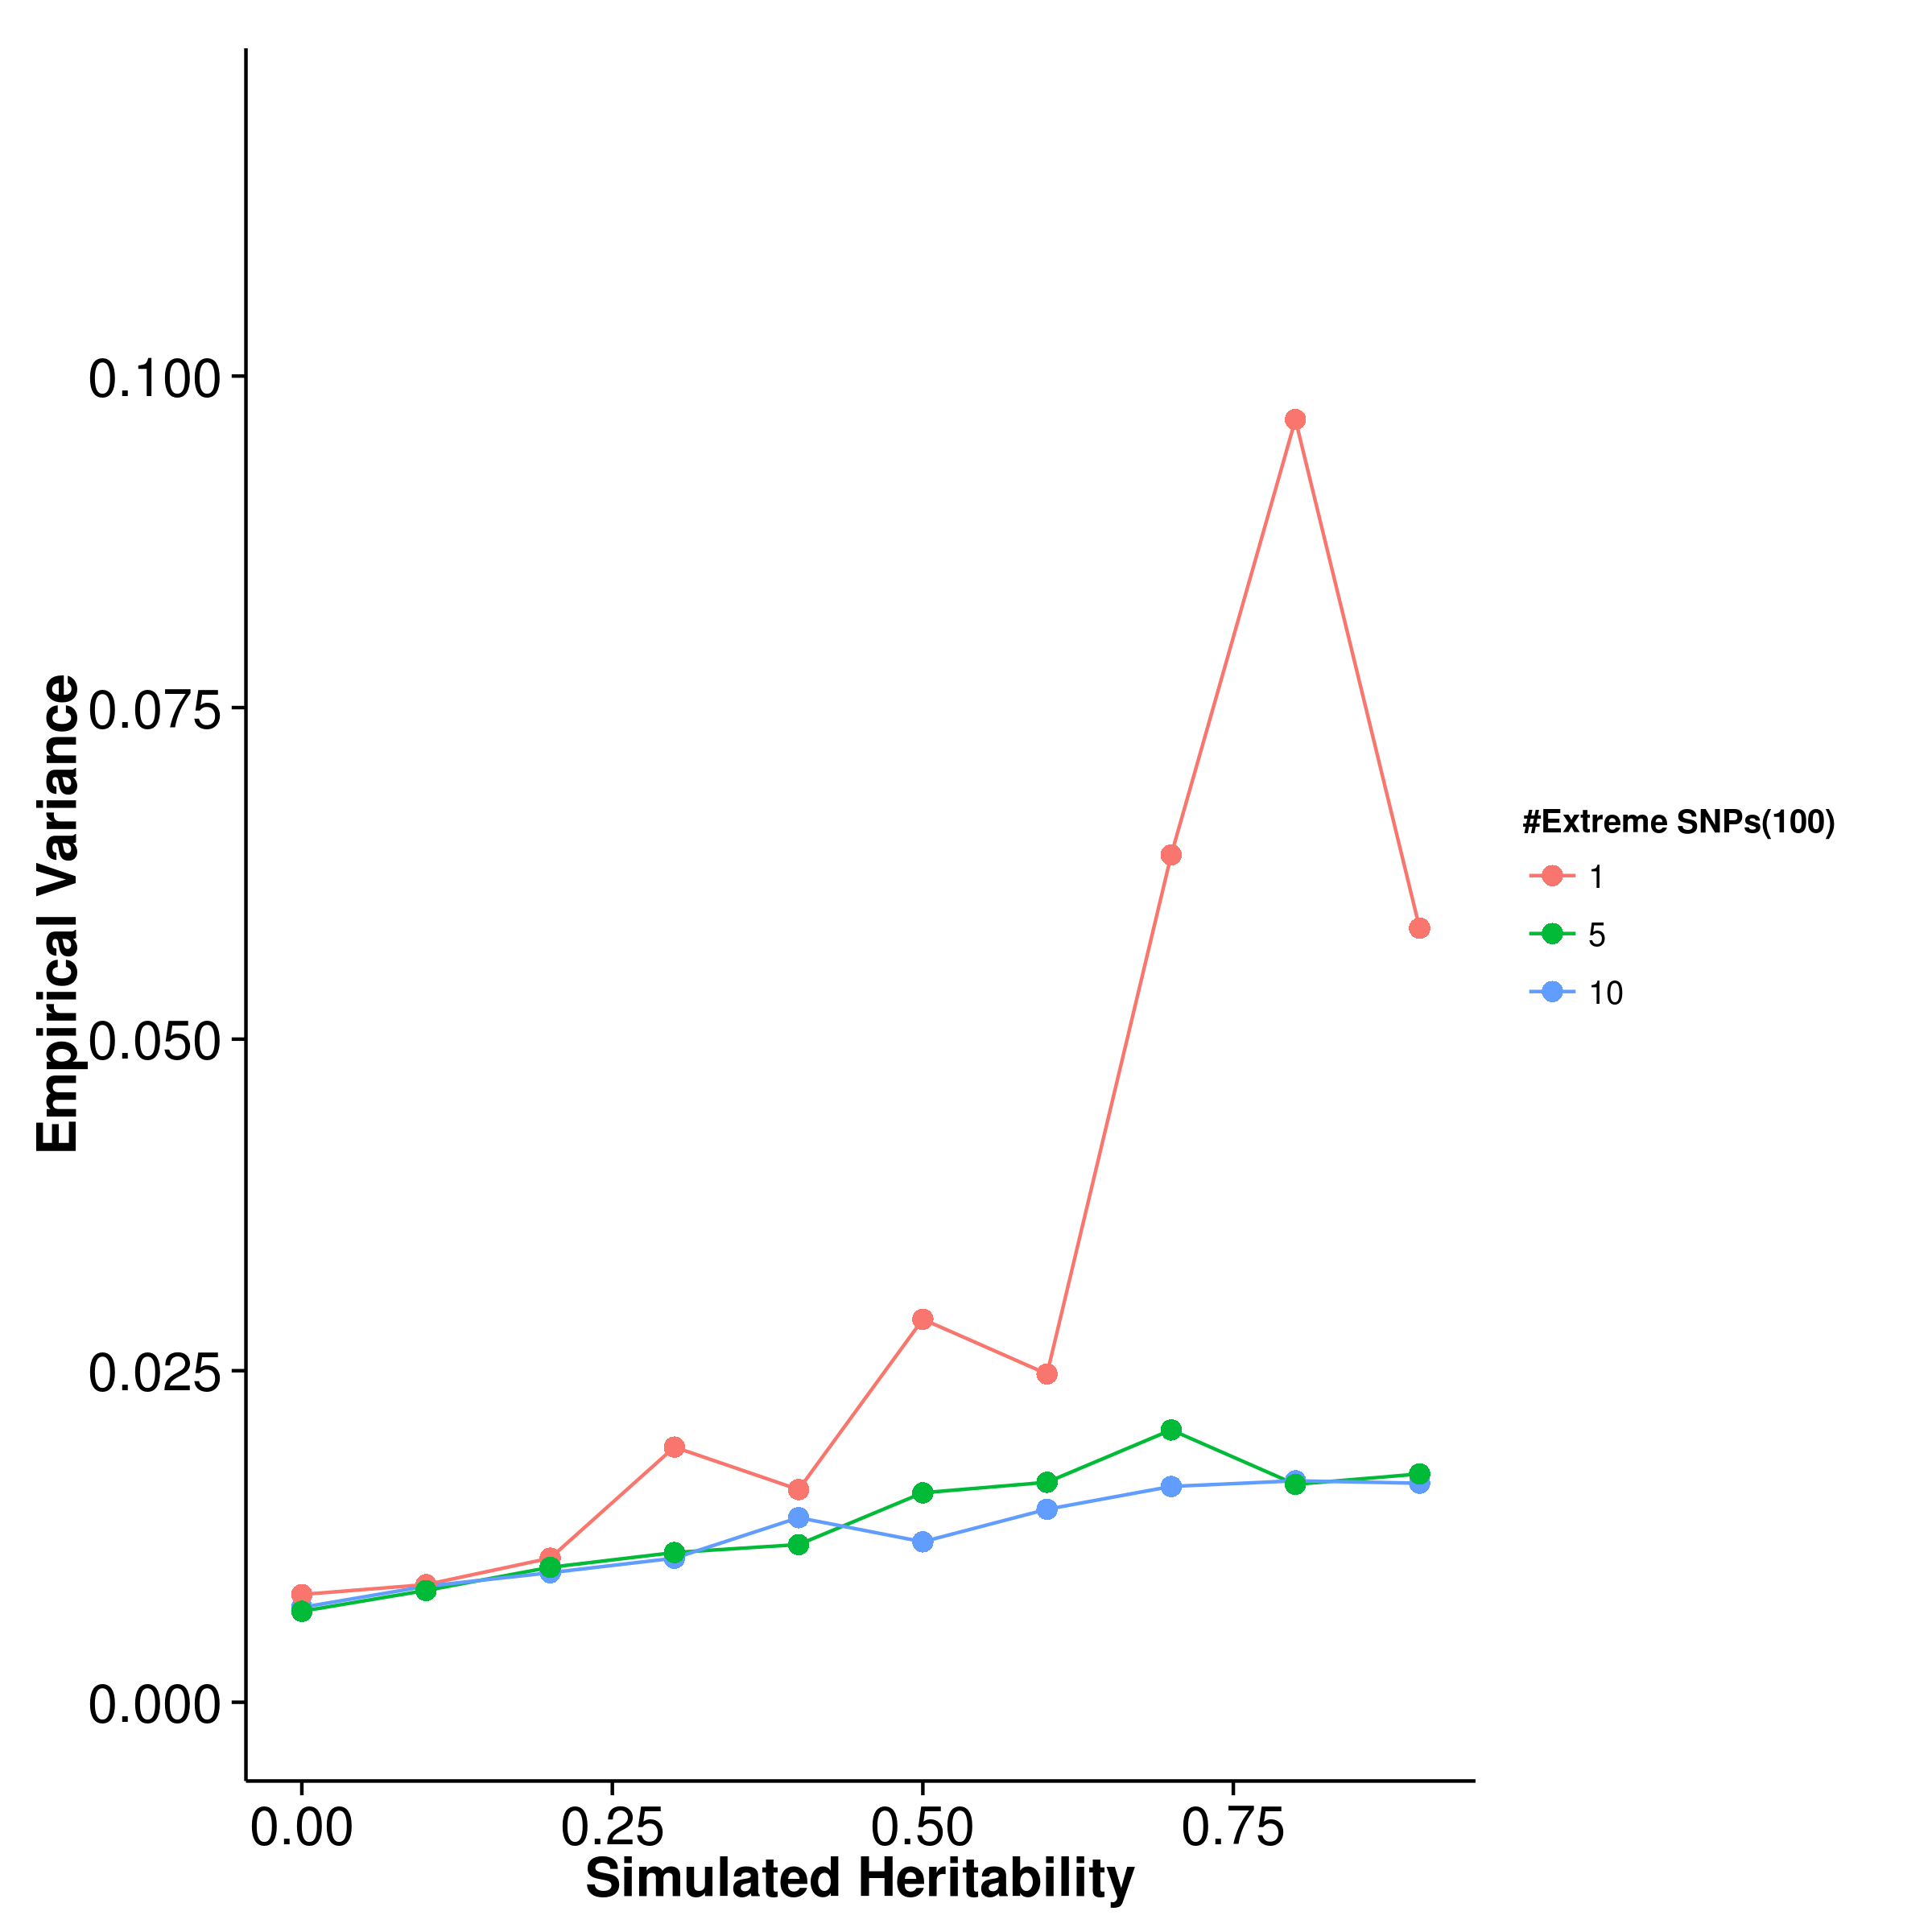
\includegraphics{figure/he_summary/extreme_100c/ldsc_QtE_Rand_sd.png}}
				\label{fig:ldscQtEx100cVar}
			}
			\subfloat[LDSC with intercept estimation]{
				
				\scalebox{.4}{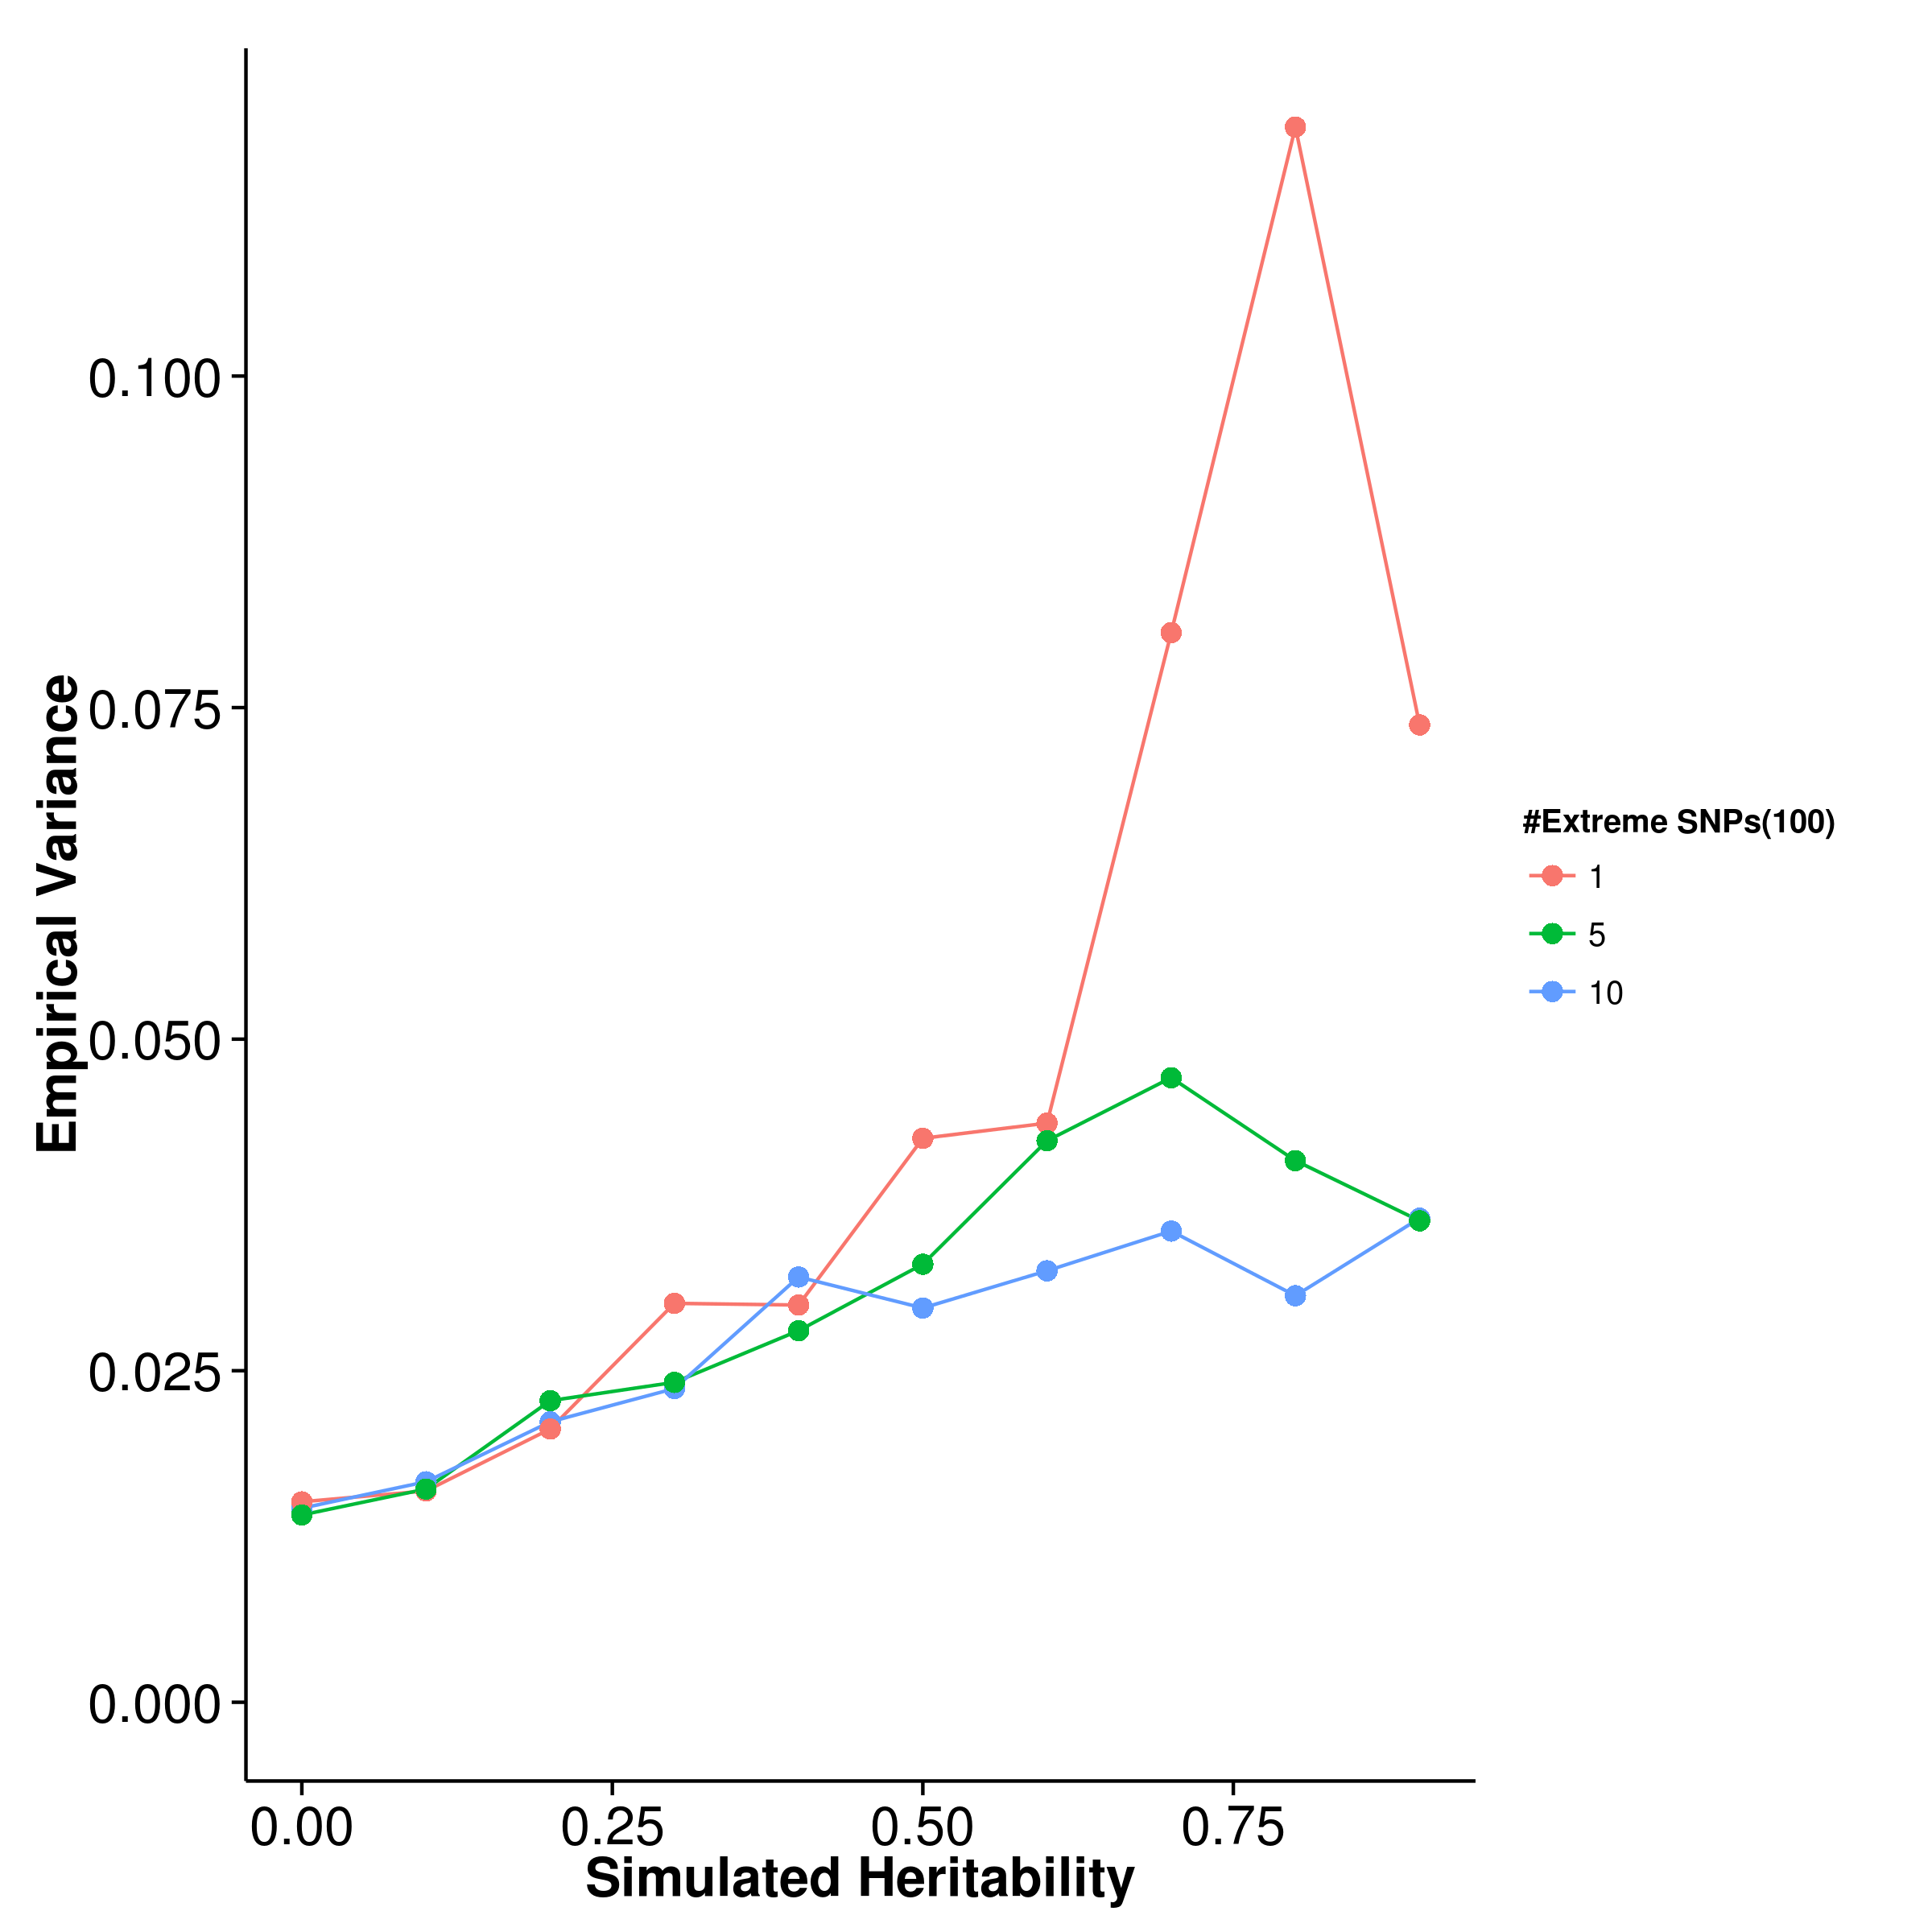
\includegraphics{figure/he_summary/extreme_100c/ldscIn_QtE_Rand_sd.png}}
				\label{fig:ldscInQtEx100cVar}
			}
			\caption[Variance of Extreme Effect Size Simulation Result]
			{Variance of results from quantitative trait simulation with extreme effect size simulation.
				100 causal \glspl{SNP} were simulated.
				When only 1 \gls{SNP} with extreme effect was simulated, the empirical variance of \gls{gcta} and \gls{ldsc} increases and a large fluctuation was observed.
				Whereas the empirical variance of \gls{shrek} only increase slightly when the simulated heritability is large and with only 1 \gls{SNP} with extreme effect.
				Suggesting that it is more robust to the change in number of extreme \gls{SNP}(s).
			} 
			\label{fig:QtEx100cVar}
		\end{figure}
		
		\begin{figure}
			\centering
			\subfloat[SHREK]{
				\scalebox{.4}{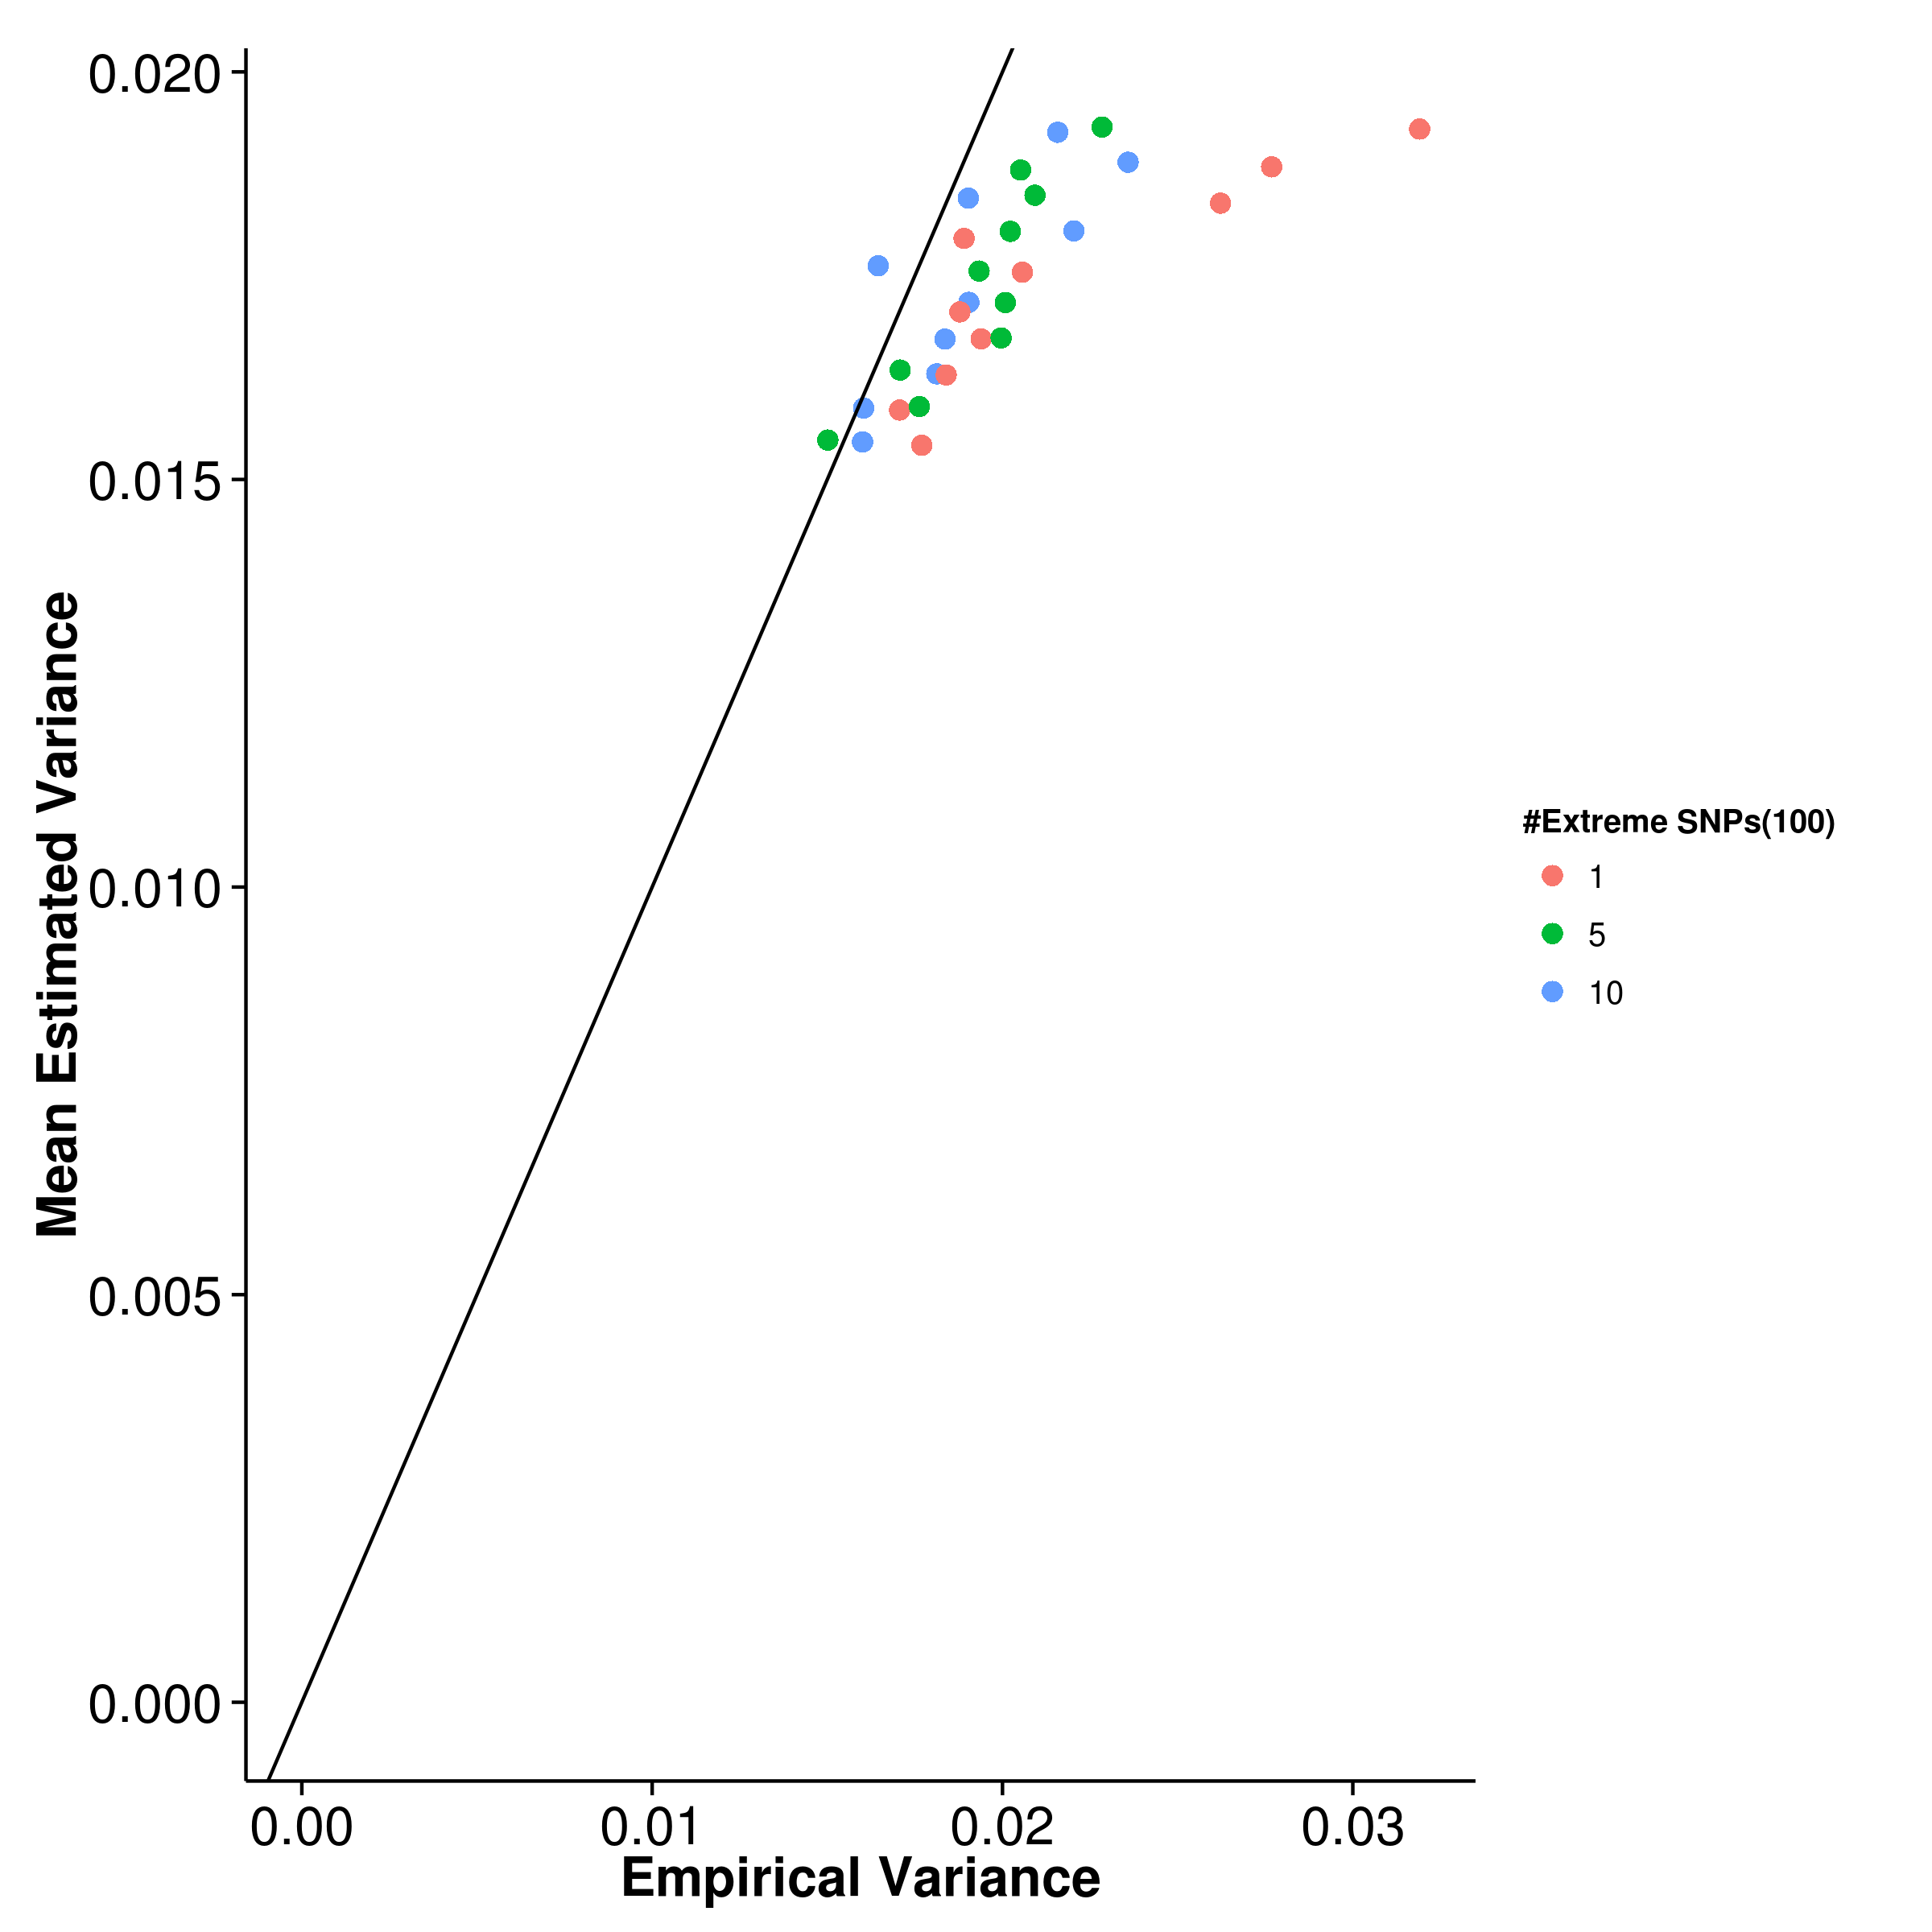
\includegraphics{figure/he_summary/extreme_100c/shrek_QtE_Rand_sdCom.png}}
				\label{fig:shrekQtEx100cVarCom}
			}
			\subfloat[GCTA]{
				\scalebox{.4}{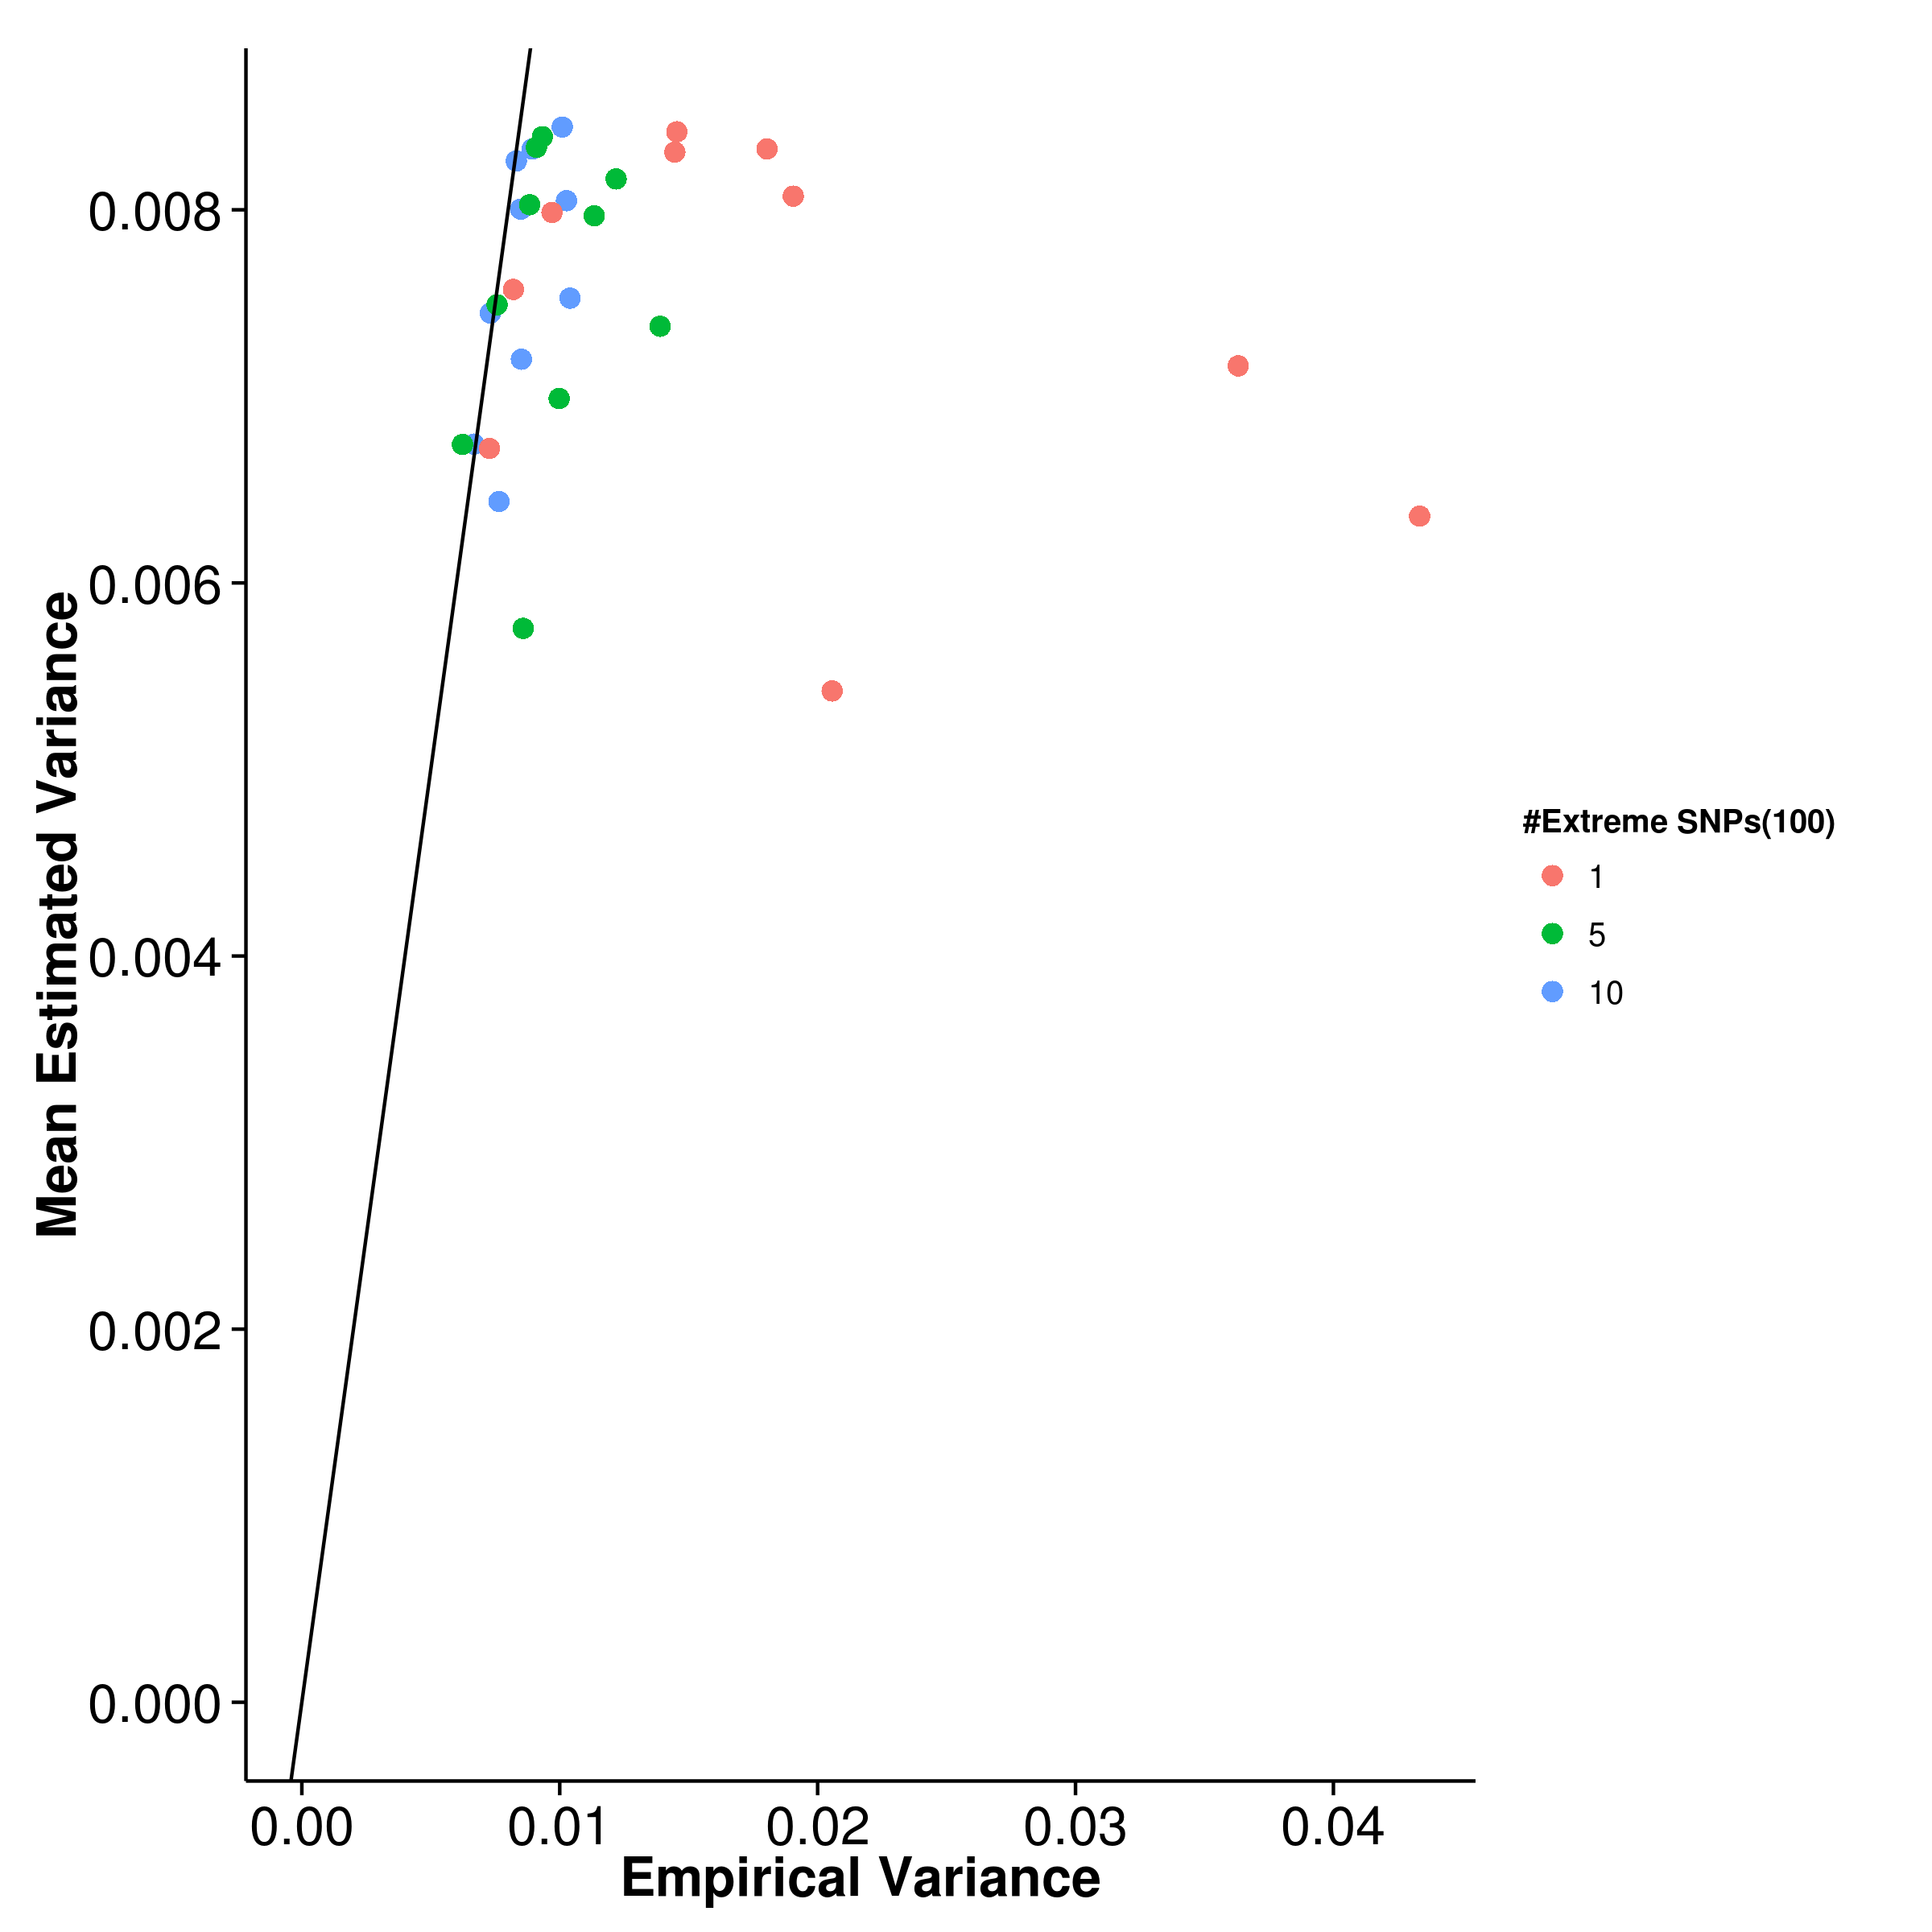
\includegraphics{figure/he_summary/extreme_100c/gcta_QtE_Rand_sdCom.png}}
				\label{fig:gctaQtEx100cVarCom}
			}\\
			\subfloat[LDSC with fix intercept]{
				\scalebox{.4}{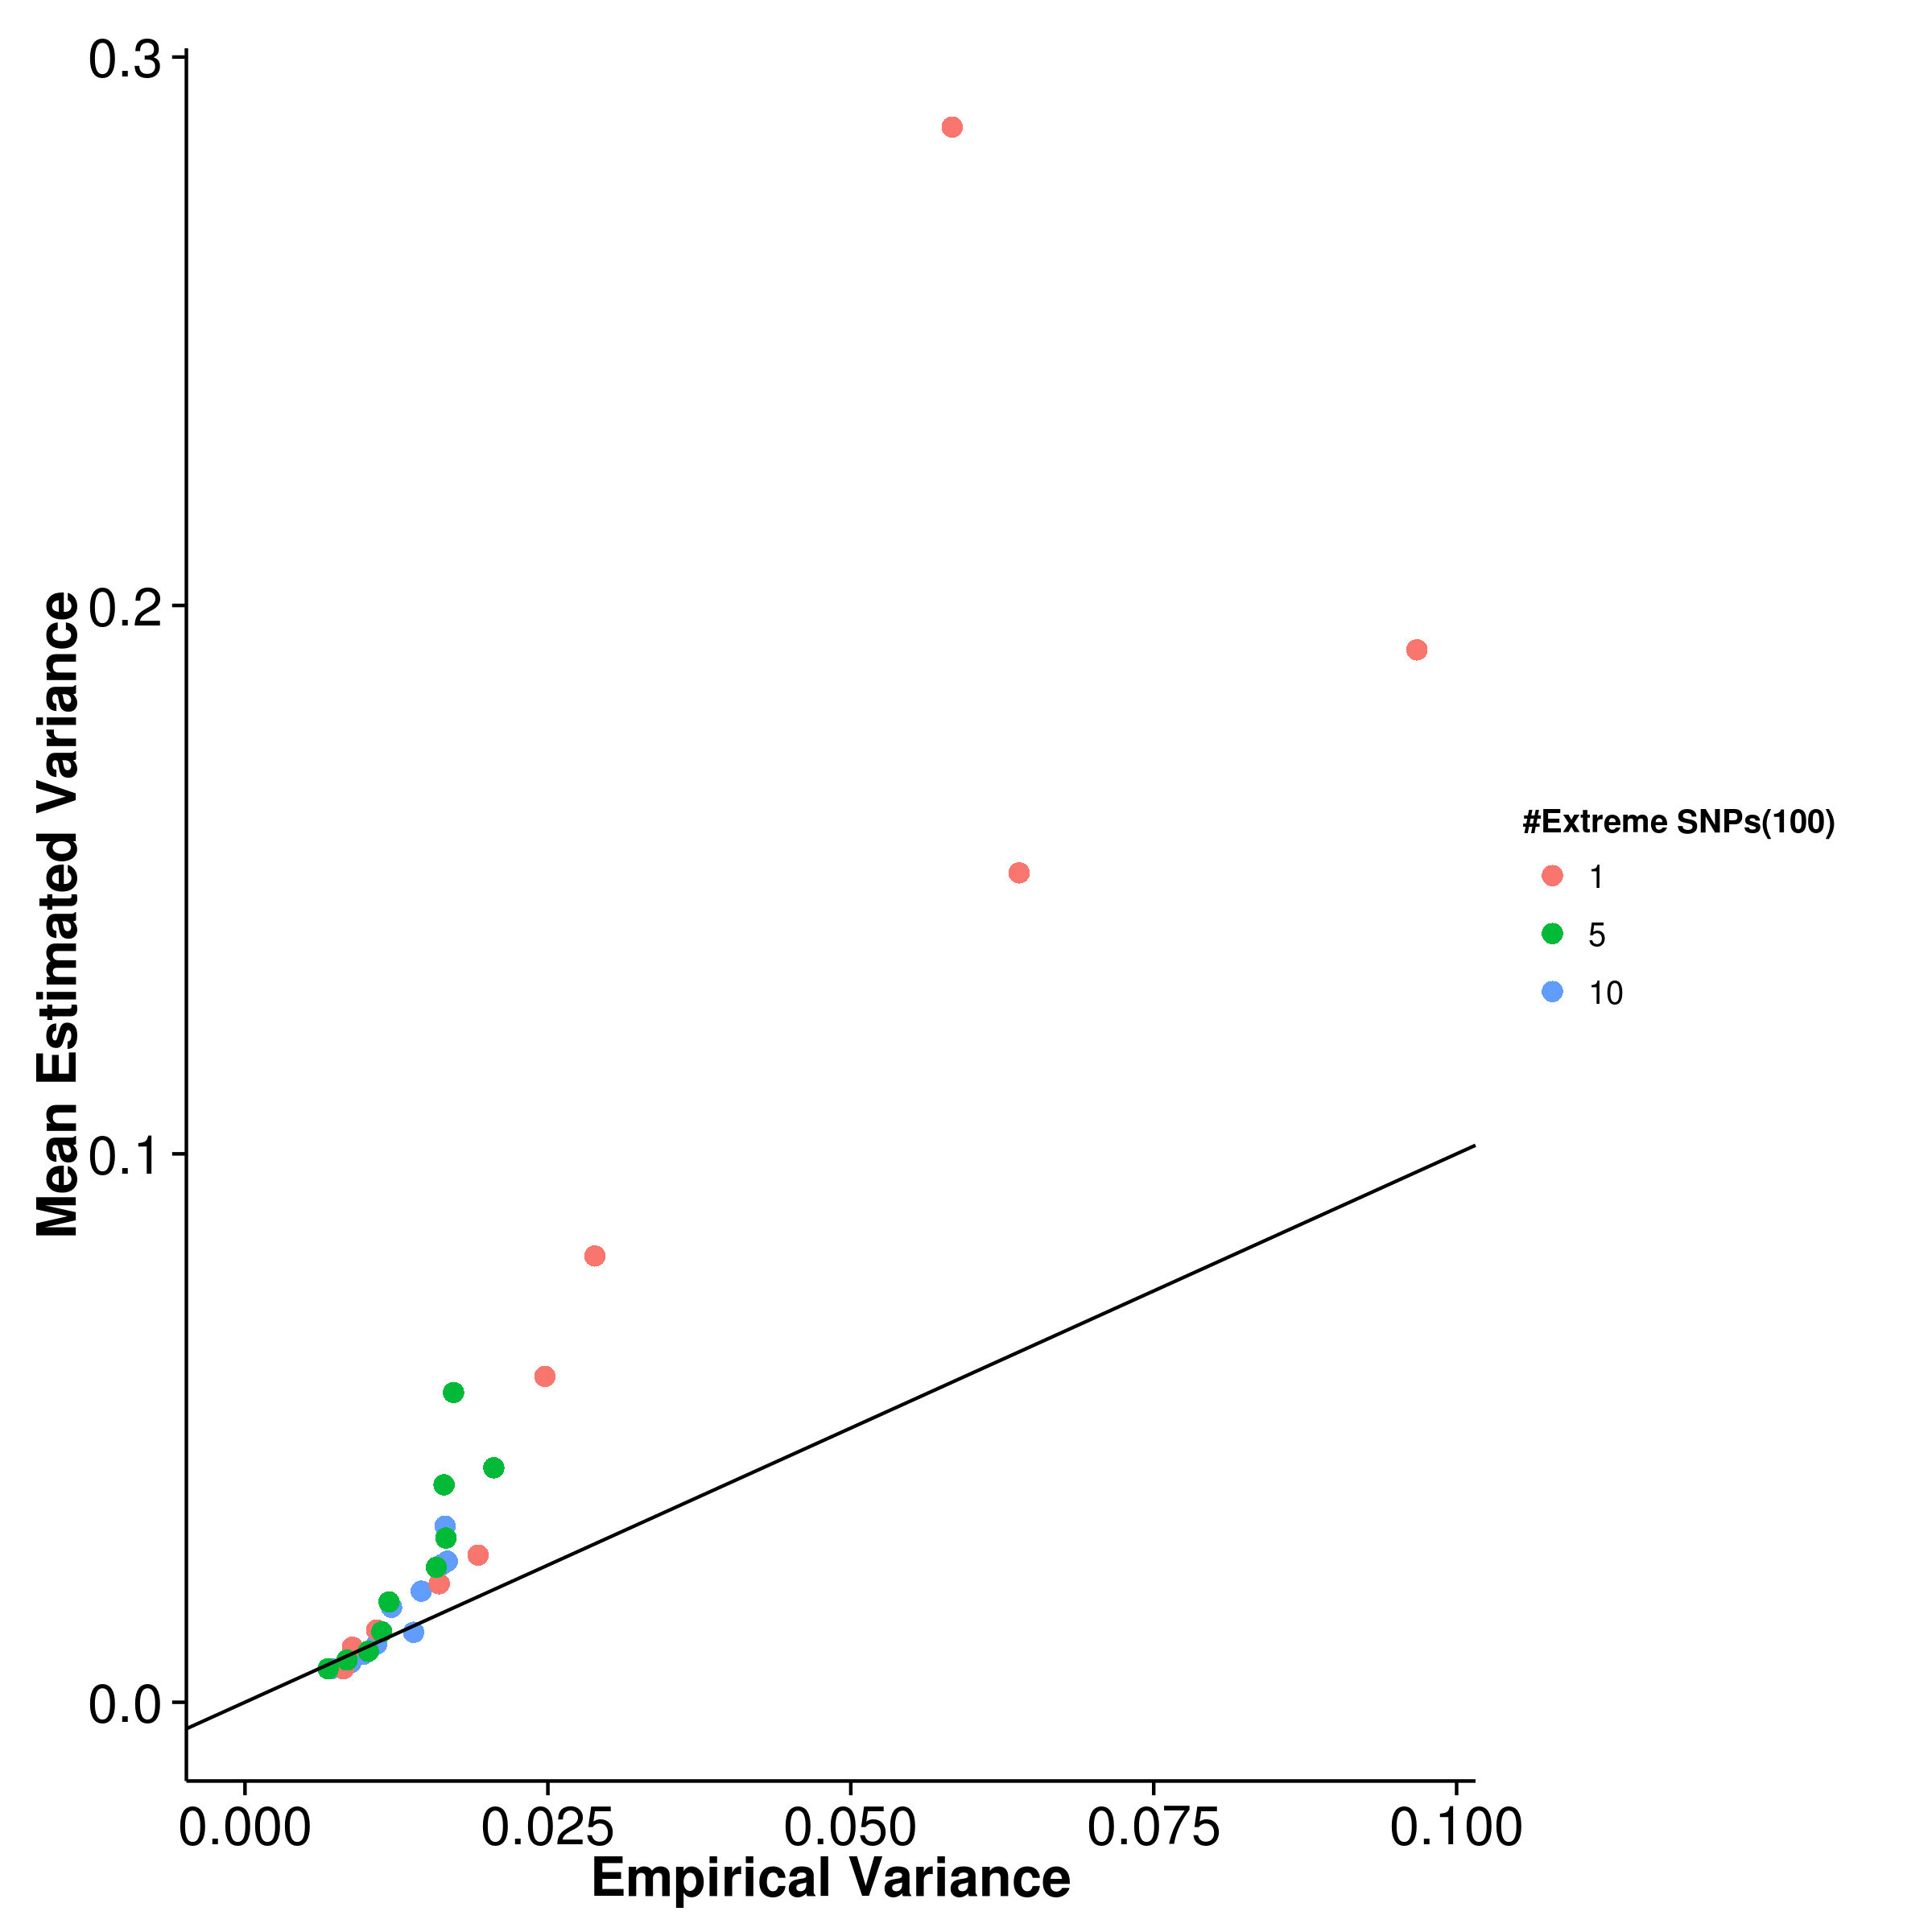
\includegraphics{figure/he_summary/extreme_100c/ldsc_QtE_Rand_sdCom.png}}
				\label{fig:ldscQtEx100cVarCom}
			}
			\subfloat[LDSC with intercept estimation]{
				
				\scalebox{.4}{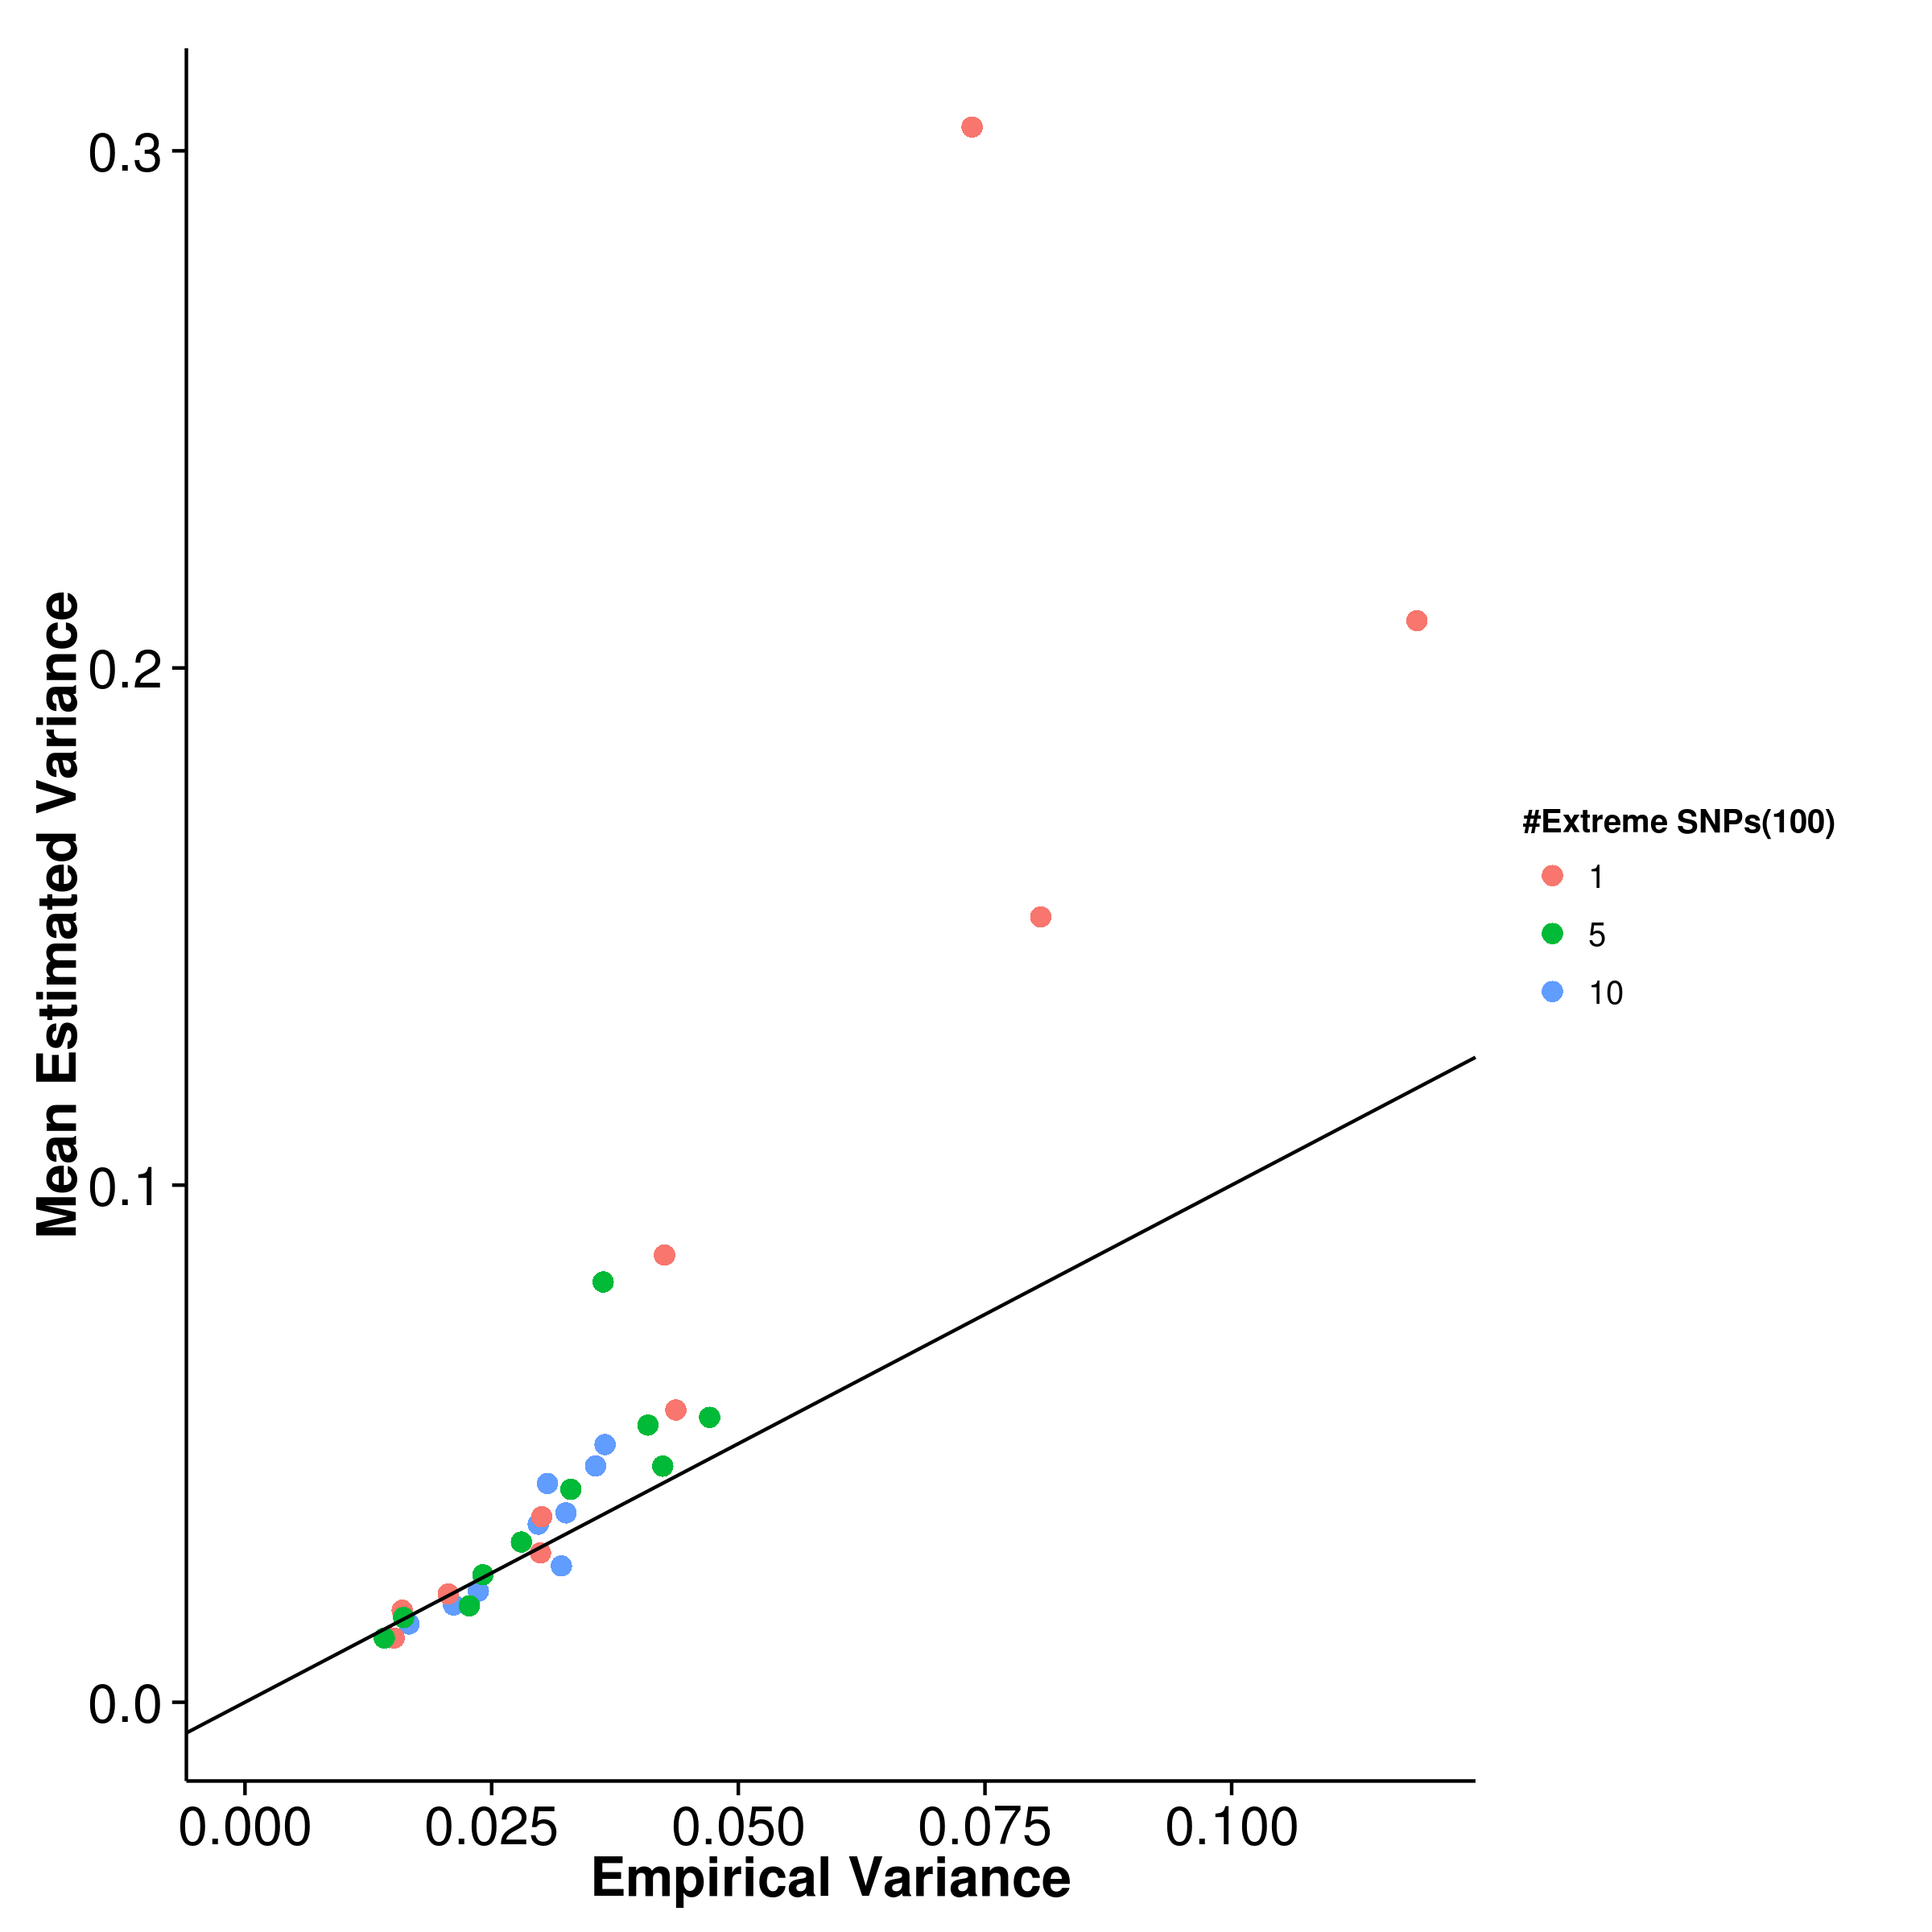
\includegraphics{figure/he_summary/extreme_100c/ldscIn_QtE_Rand_sdCom.png}}
				\label{fig:ldscInQtEx100cVarCom}
			}
			\caption[Estimation of Variance in Extreme Effect Size Simulation]
			{Estimated variance of results from quantitative trait simulation with extreme effect size simulation when compared to the empirical variance.
				100 causal \glspl{SNP} were simulated.
				\gls{shrek} and \gls{gcta} generally under-estimate the variance with the magnitude of bias being the highest when there is only 1 \gls{SNP} with extreme effect.
				On the other hand, \gls{ldsc} tends to over-estimate the variance and it can overestimate the variance by more than 3 folds when there is only 1 \gls{SNP} with extreme effect.
			} 
			\label{fig:QtEx100cVarCom}
		\end{figure}